\begin{frame}{Track Positions (x, y)}
    \centering
    % \underline{Basic Plot Parameters}
    \begin{itemize}
        \item Vetonu
        \item VetoStation 1 [in Backup]
        \item VetoStation 2 [in Backup]
        \item Trigger/Timing Station [in Backup]
        \item Tracking Station 1
        \item Tracking Station 3
        \item Preshower 1 [in Backup]
        \item Preshower 2 [in Backup]
        \item Calo
        \item Max Radius
    \end{itemize}
\end{frame}

\begin{frame}{Track Positions at Vetonu}
    \begin{columns}
        \begin{column}{0.5\textwidth}
            \begin{figure}
                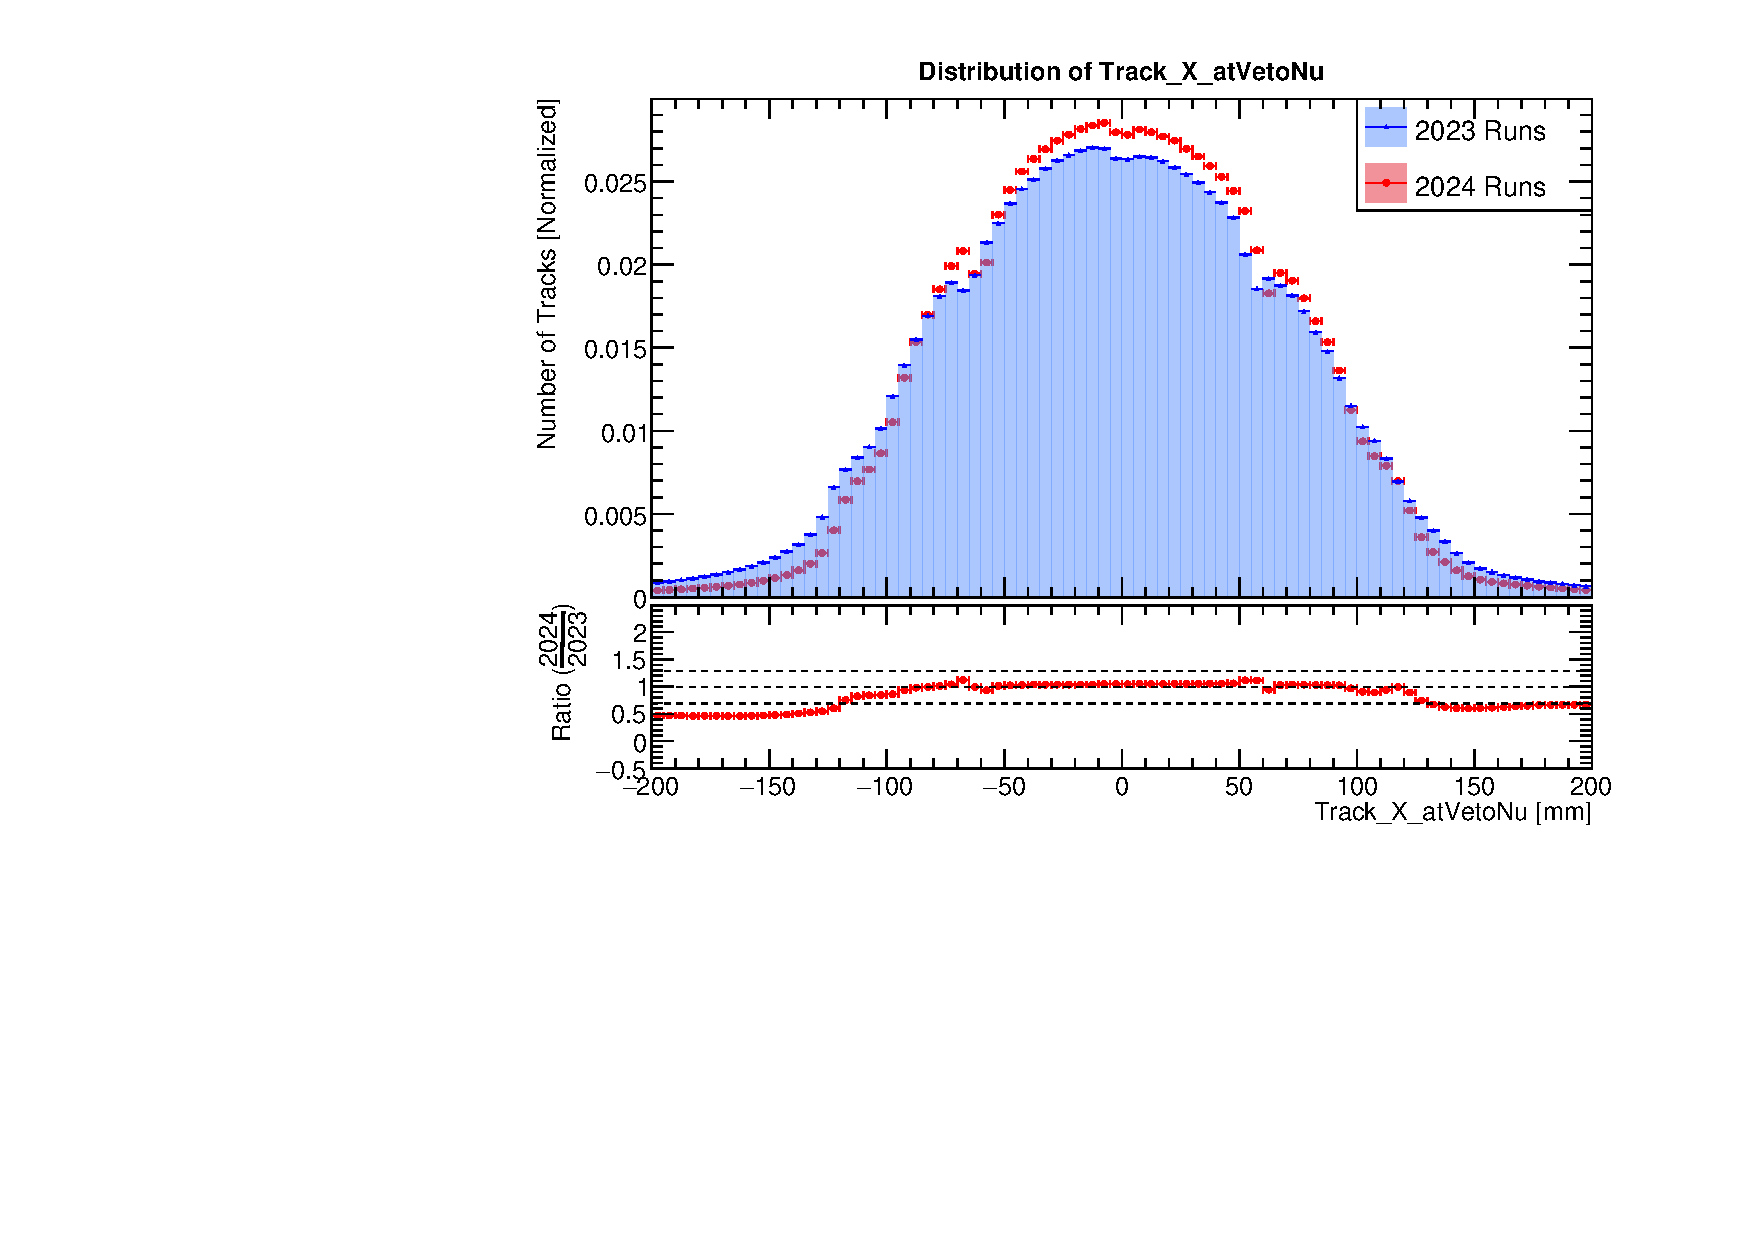
\includegraphics[width=\linewidth] {\plots/Track_X_atVetoNu.pdf}
                \caption{Track Position x at VetoNu}
            \end{figure}
        \end{column}
        \begin{column}{0.5\textwidth}
            \begin{figure}
                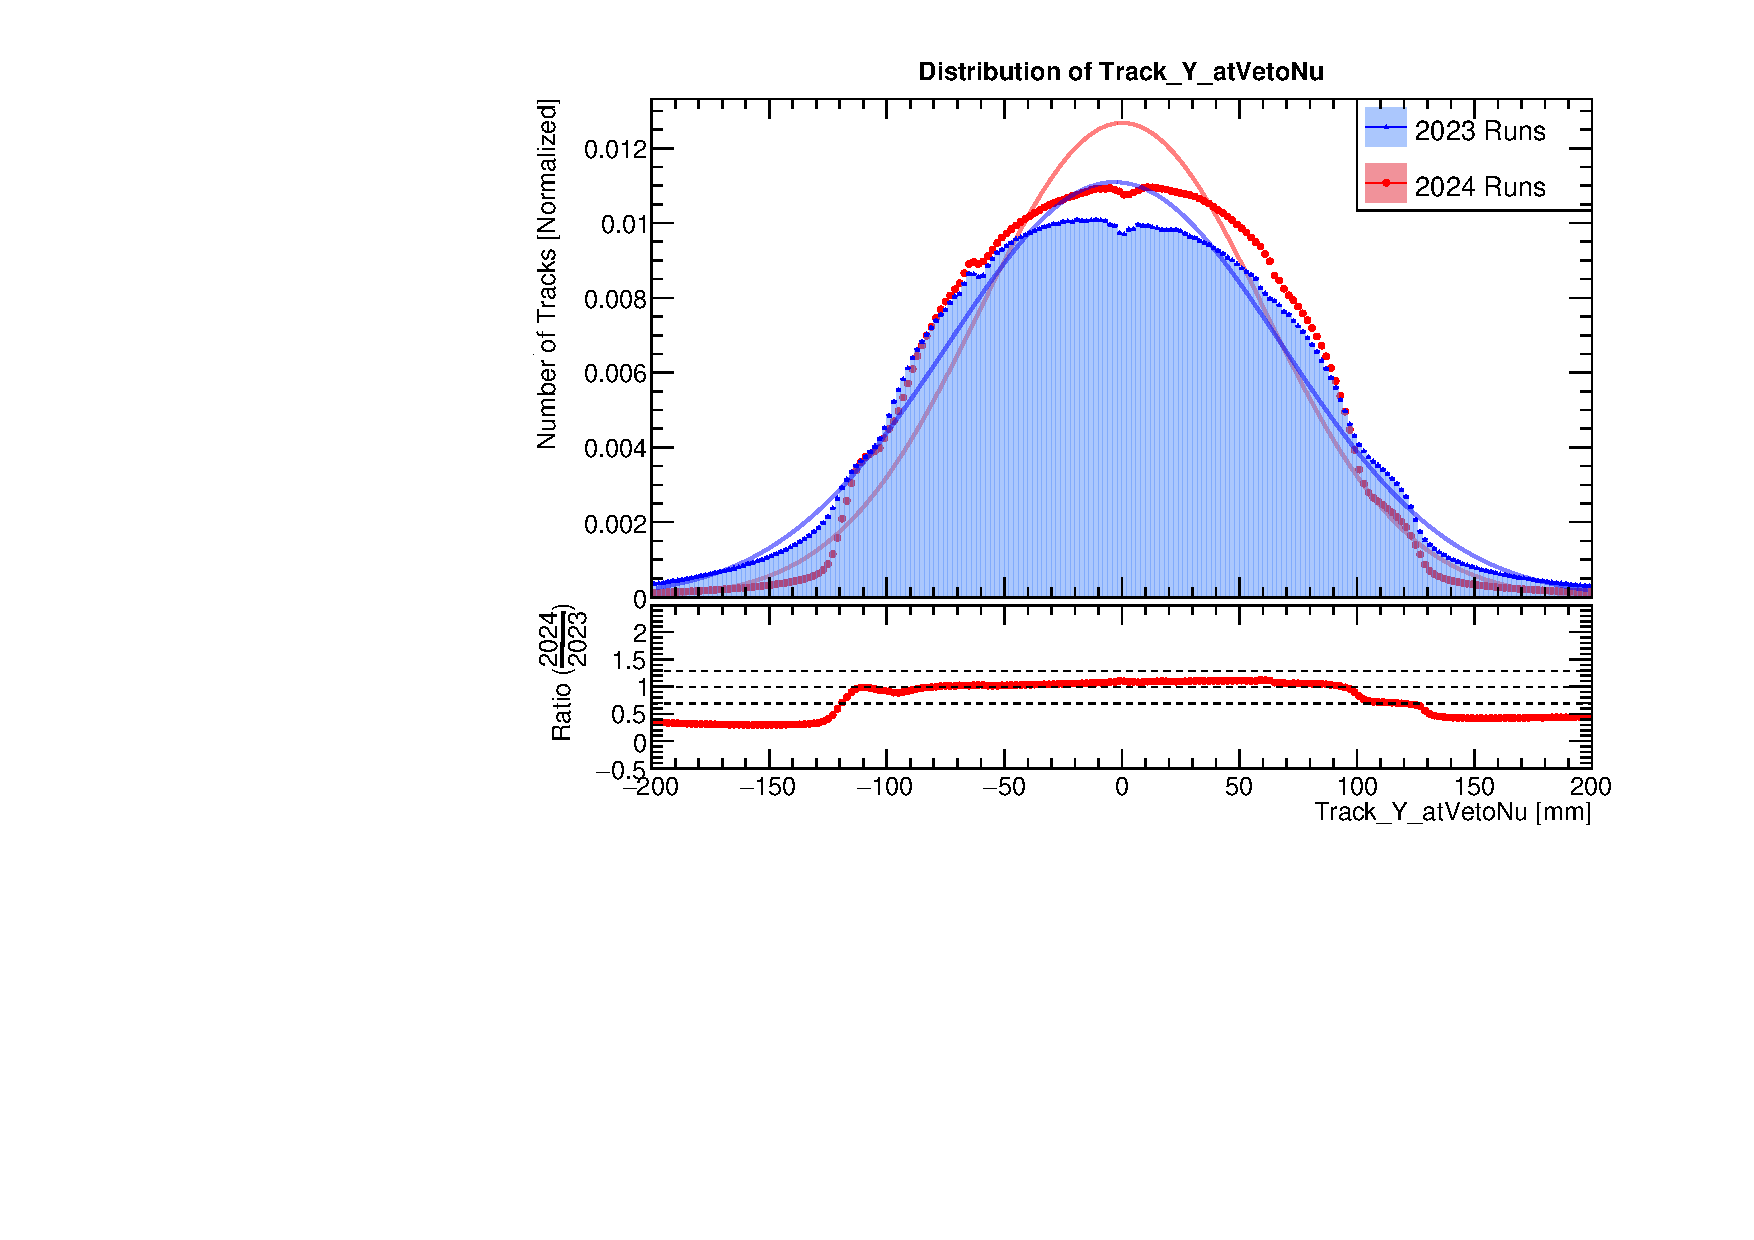
\includegraphics[width=\linewidth] {\plots/Track_Y_atVetoNu.pdf}
                \caption{Track Position y at VetoNu}
            \end{figure}
        \end{column}
    \end{columns}
    \begin{itemize}
        \item Sharper Distribution in 2024: More particles on center? REF?
              % \item The ypeak has shifted from -12.5 mm to 12.5 mm.
        \item The ypeak has shifted to the positive side. Expected with the change in beam crossing angle
        % \item Beam crossing angle went 160 $\mu$Rad downward to 160 $\mu$Rad upwards. Thus we
            %   expect the peak y positions to go from negative to positive
        % \item Offset went from [6.5 cm CHECK THIS?] Calculations show 1.18 cm.
        \item Same comments hold for the rest of the positions.
    \end{itemize}
\end{frame}

\begin{subframe}{Track Positions at Veto Station 1 [SKIP]}
    \begin{columns}
        \begin{column}{0.5\textwidth}
            \begin{figure}
                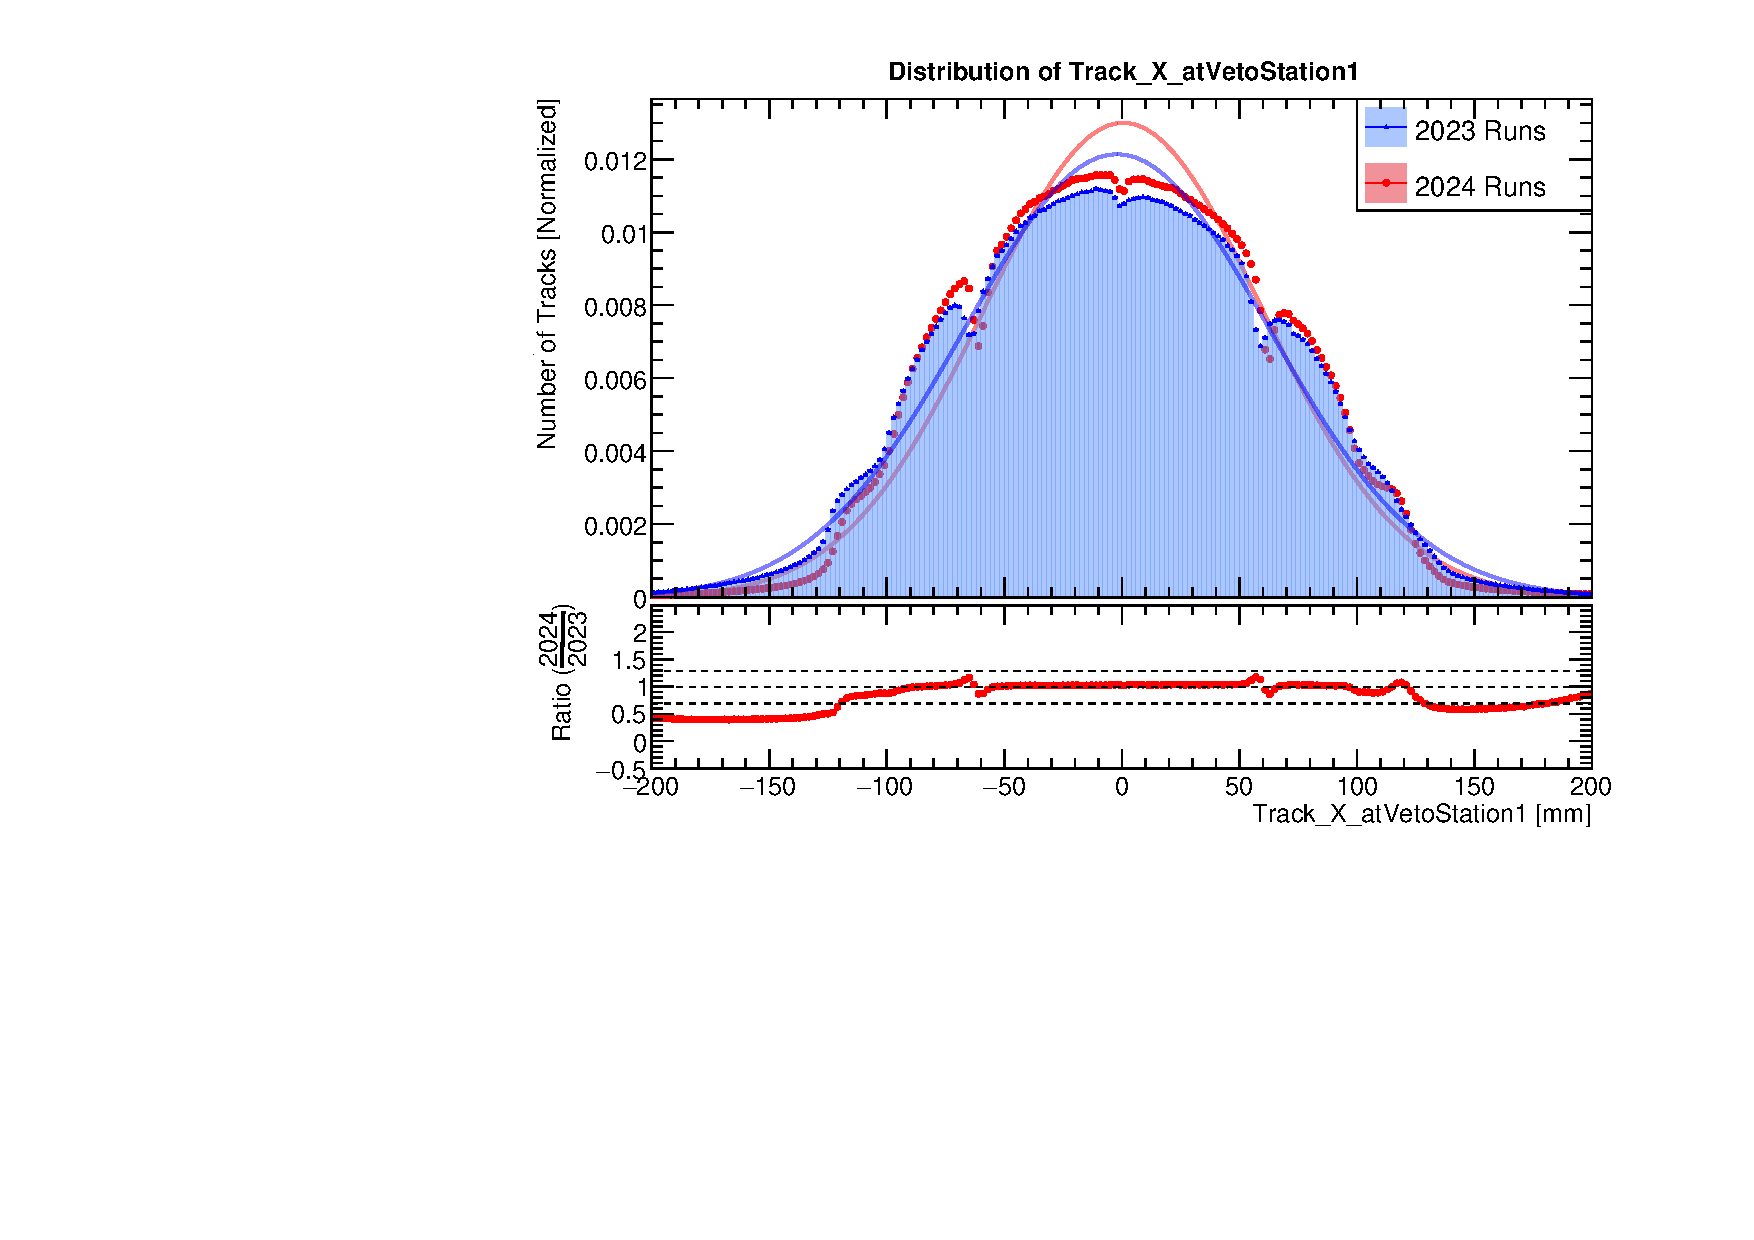
\includegraphics[width=\linewidth] {\plots/Track_X_atVetoStation1.pdf}
                \caption{Track Position x at Veto Station 1}
            \end{figure}
        \end{column}
        \begin{column}{0.5\textwidth}
            \begin{figure}
                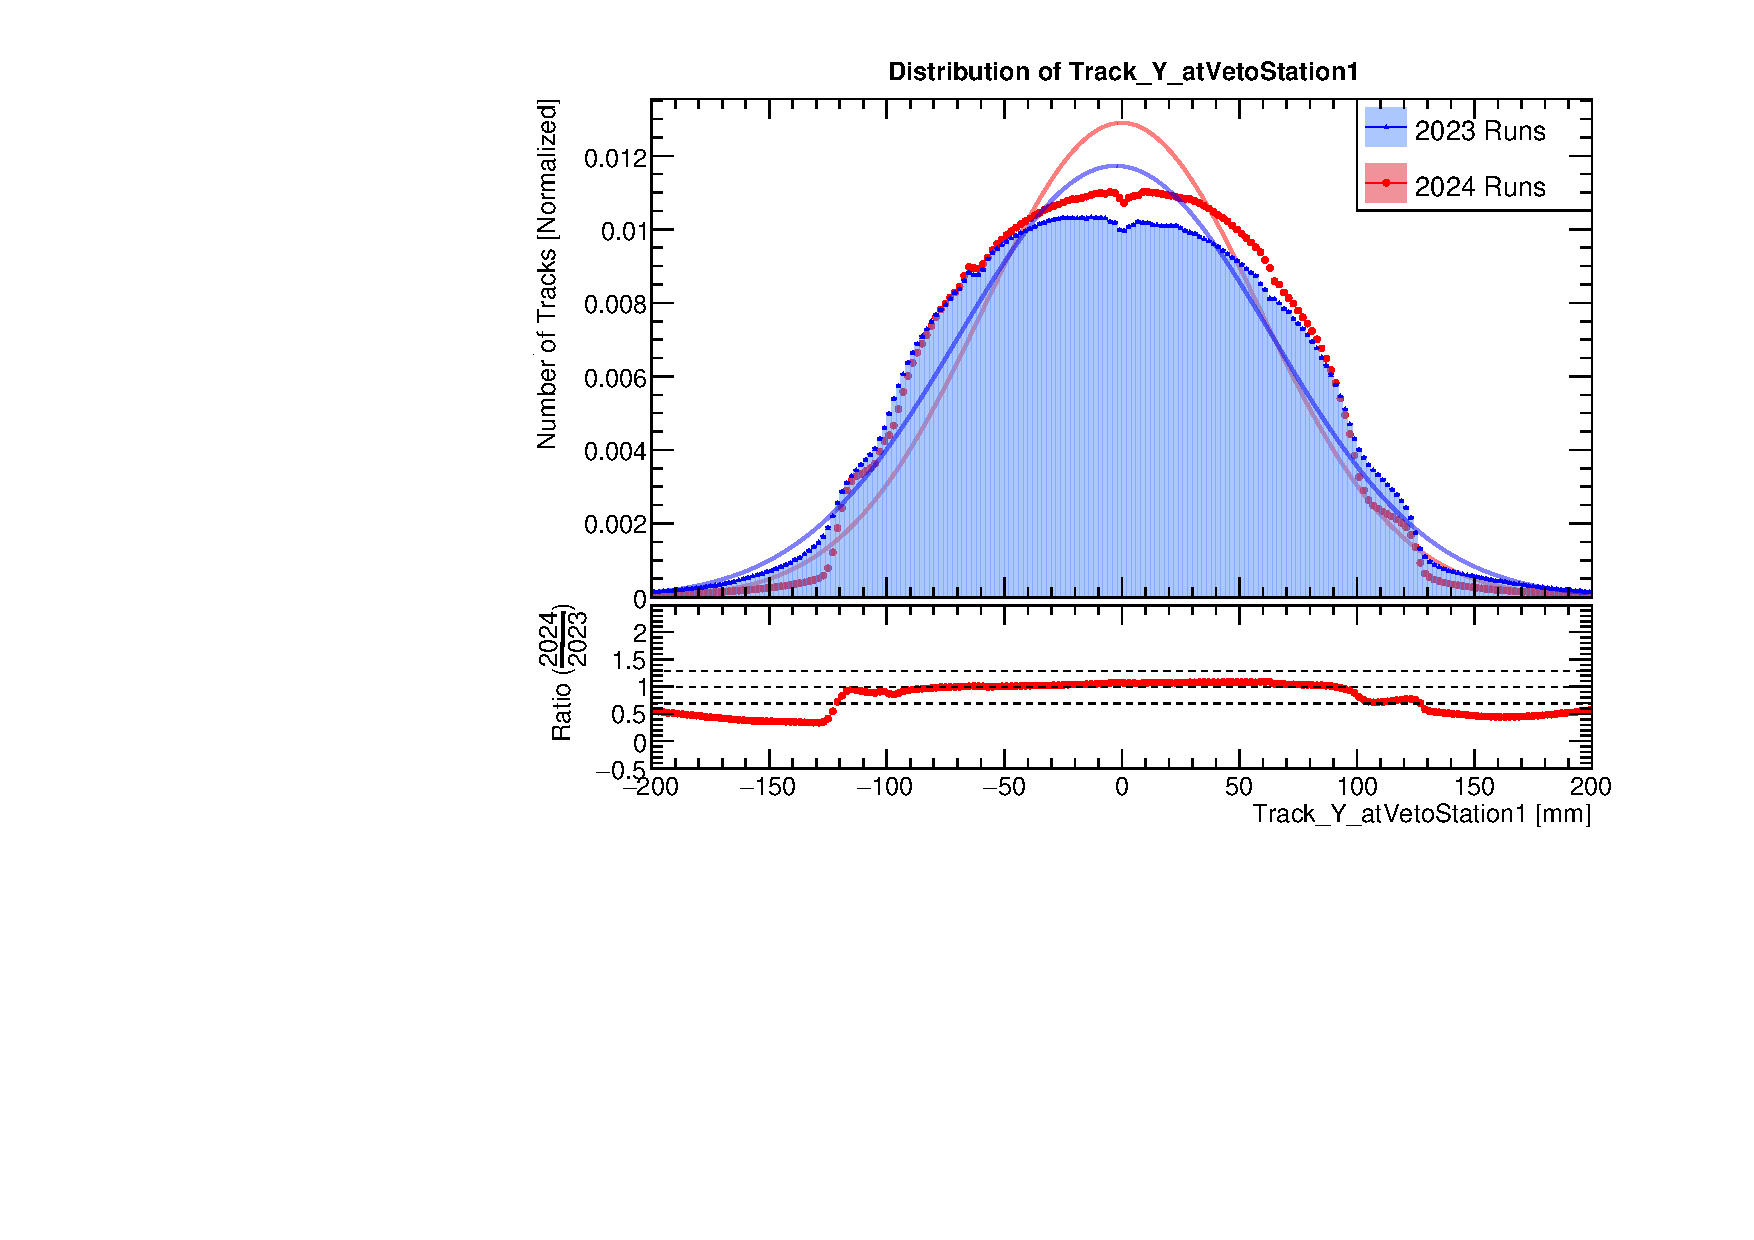
\includegraphics[width=\linewidth] {\plots/Track_Y_atVetoStation1.pdf}
                \caption{Track Position y at Veto Station 1}
            \end{figure}
        \end{column}
    \end{columns}
\end{subframe}

\begin{subframe}{Track Positions at Veto Station 2 [SKIP]}
    \begin{columns}
        \begin{column}{0.5\textwidth}
            \begin{figure}
                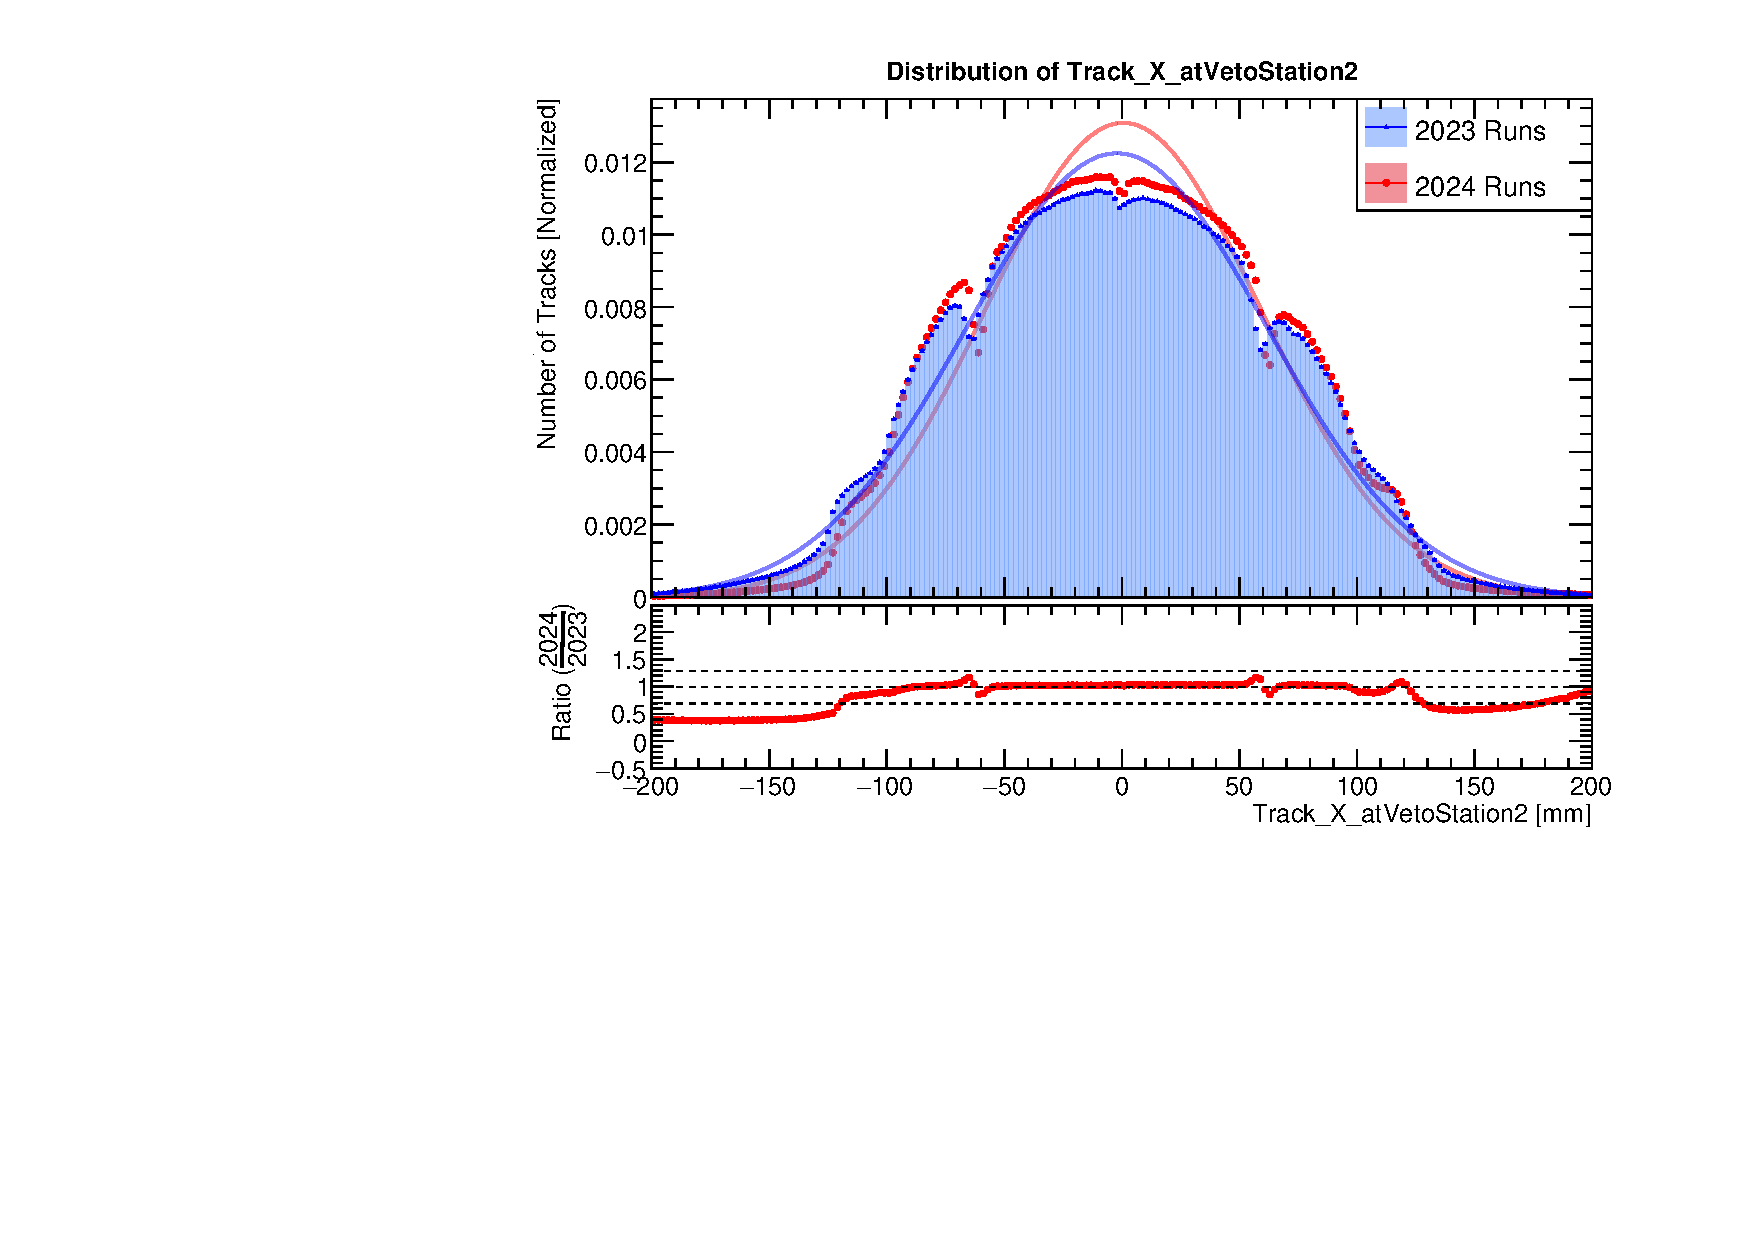
\includegraphics[width=\linewidth] {\plots/Track_X_atVetoStation2.pdf}
                \caption{Track Position x at Veto Station 2}
            \end{figure}
        \end{column}
        \begin{column}{0.5\textwidth}
            \begin{figure}
                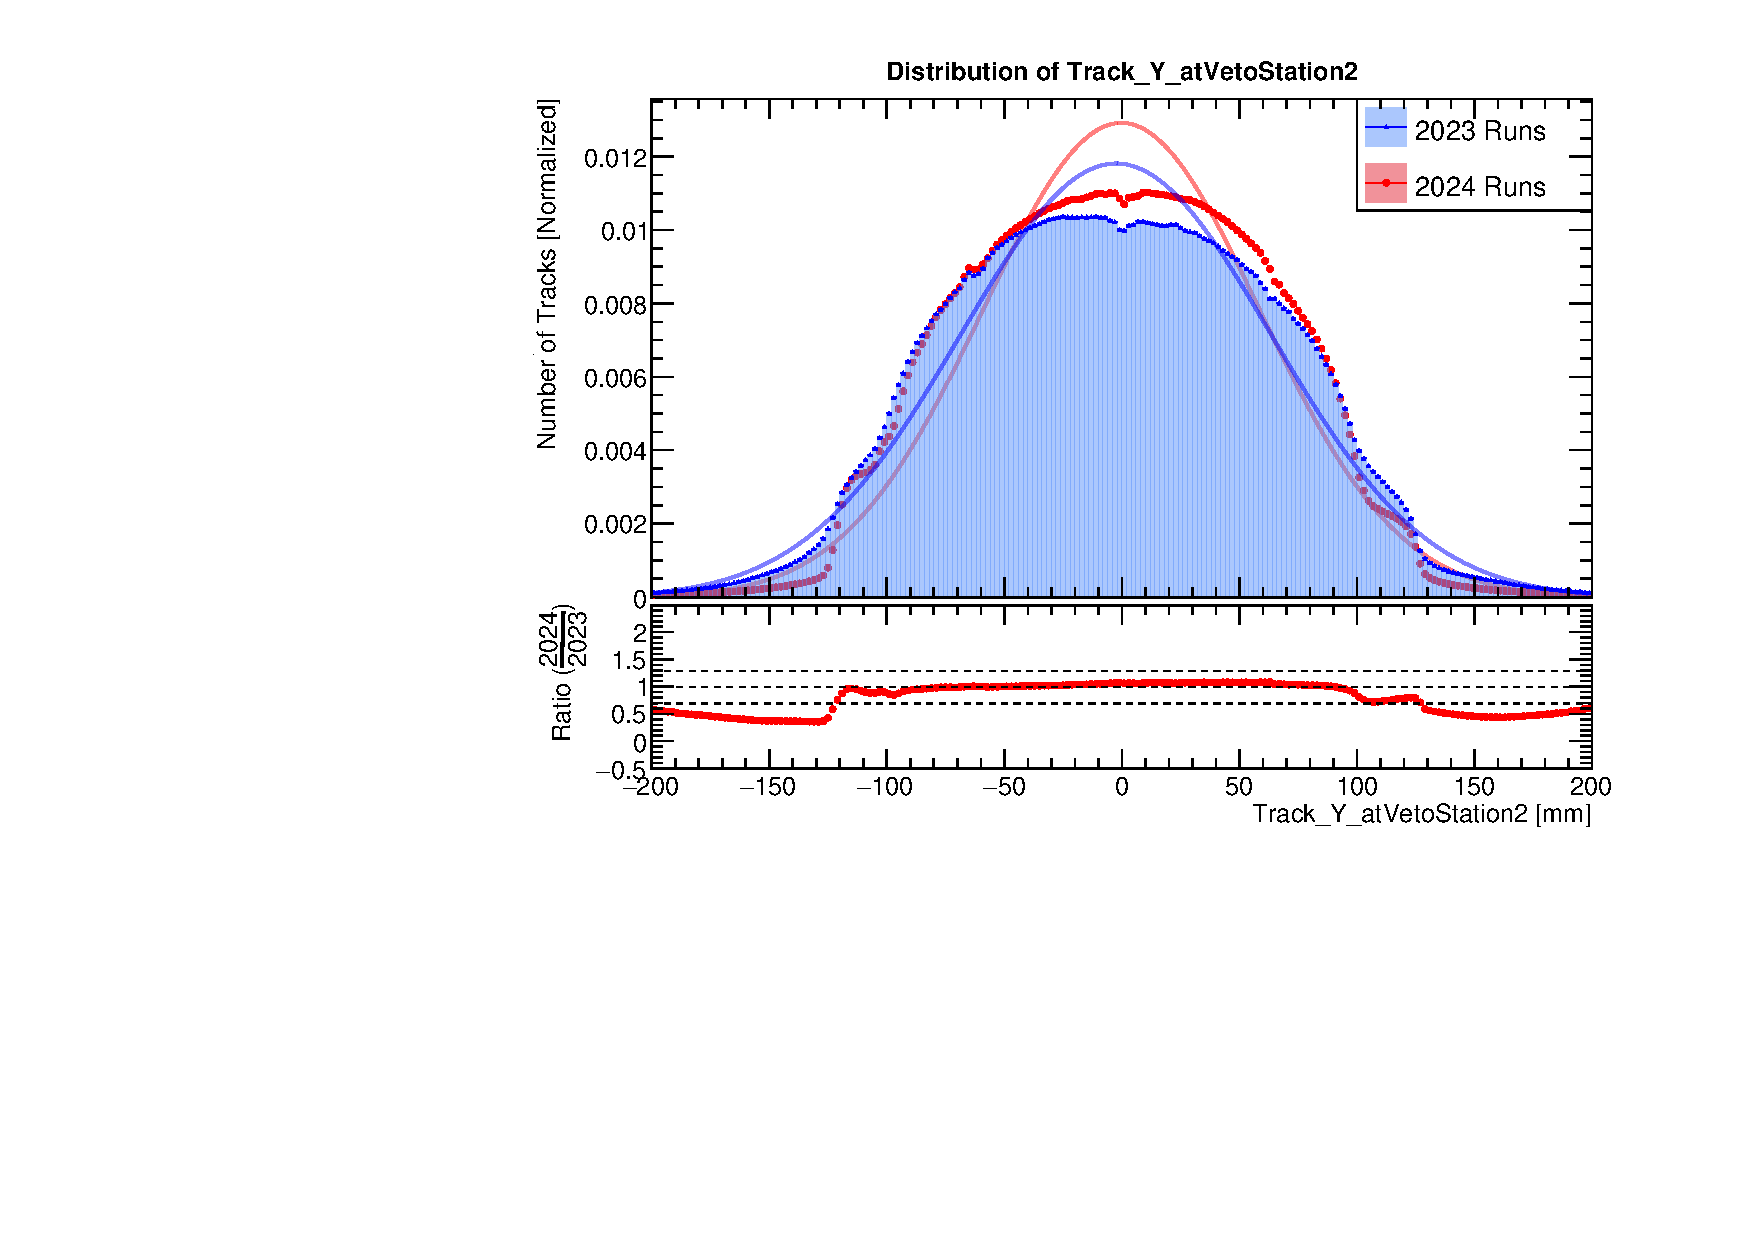
\includegraphics[width=\linewidth] {\plots/Track_Y_atVetoStation2.pdf}
                \caption{Track Position y at Veto Station 2}
            \end{figure}
        \end{column}
    \end{columns}
\end{subframe}

\begin{subframe}{Track Positions at Trigger [SKIP]}
    \begin{columns}
        \begin{column}{0.5\textwidth}
            \begin{figure}
                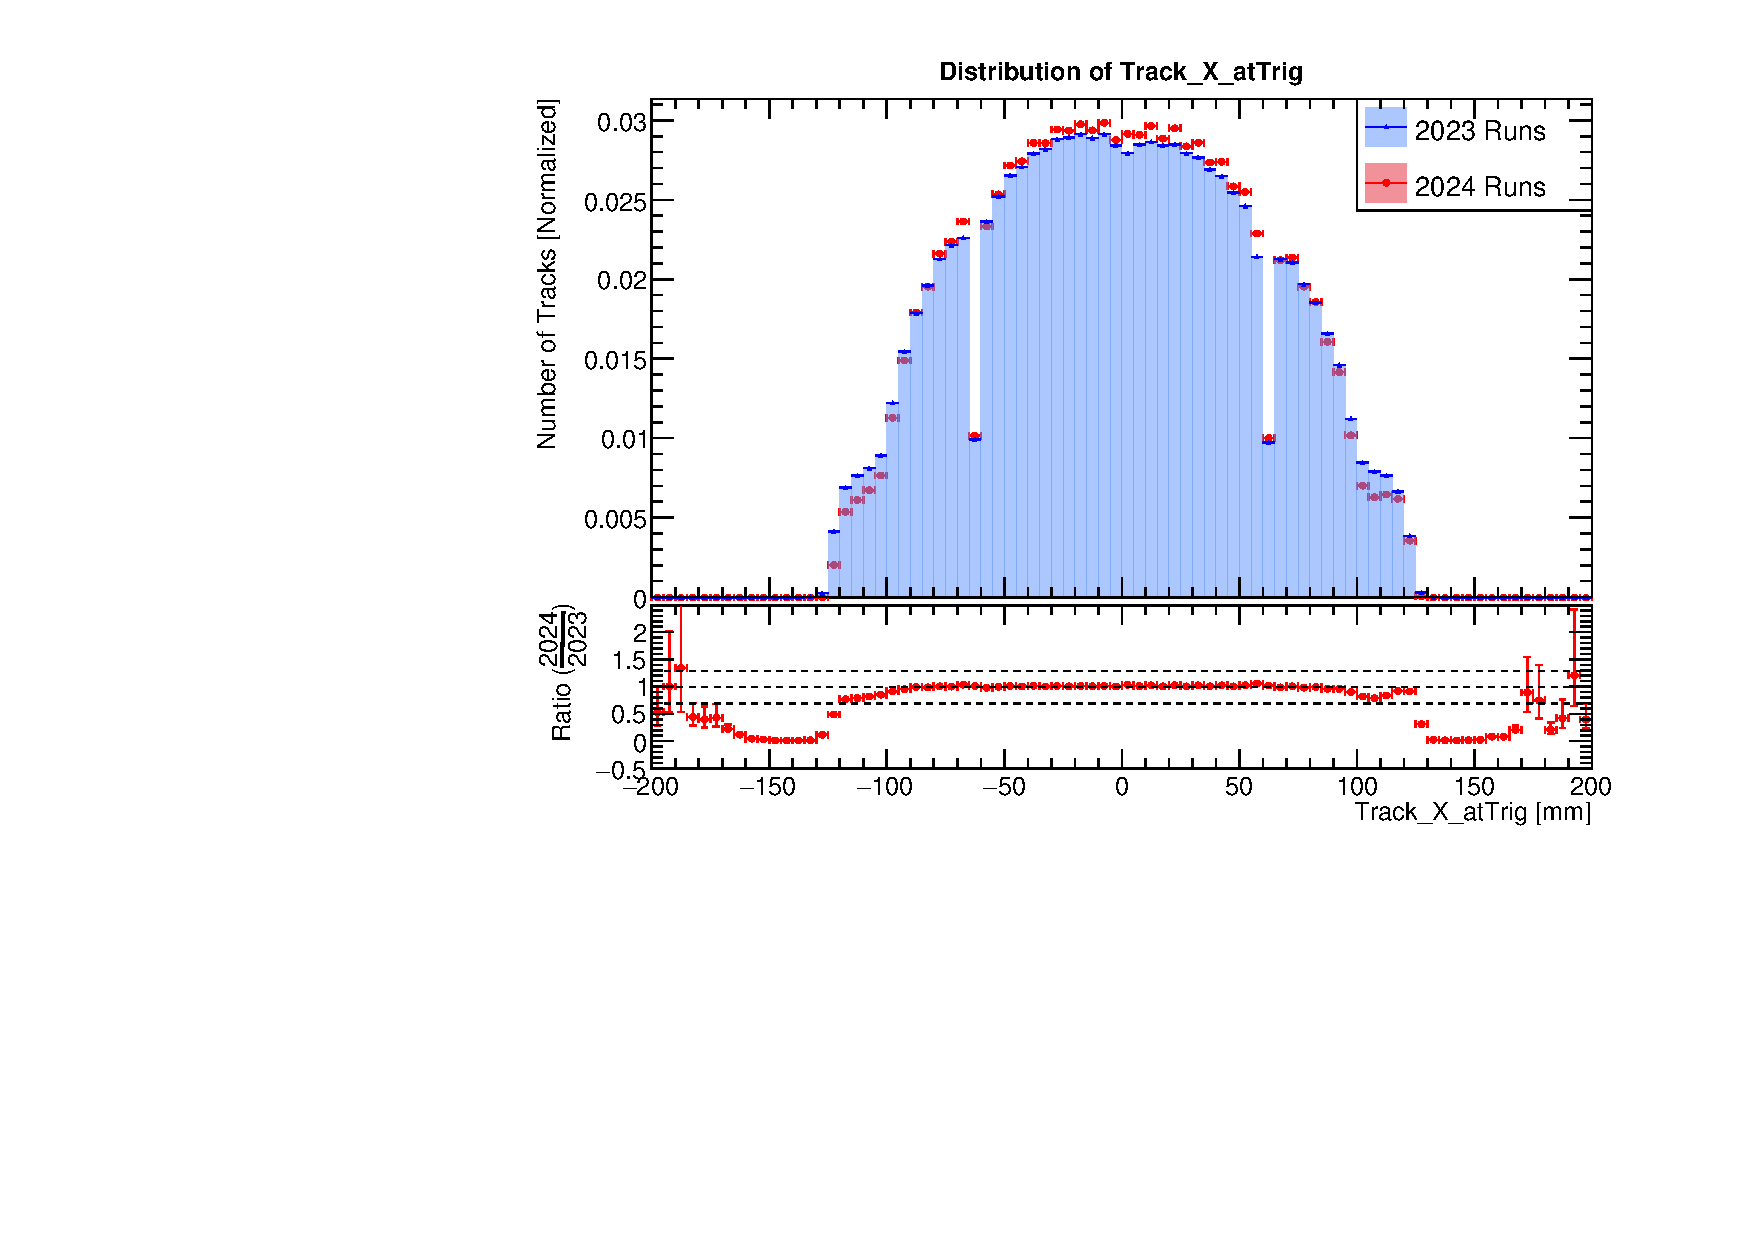
\includegraphics[width=\linewidth] {\plots/Track_X_atTrig.pdf}
                \caption{Track Position x at Trigger/Timing Station}
            \end{figure}
        \end{column}
        \begin{column}{0.5\textwidth}
            \begin{figure}
                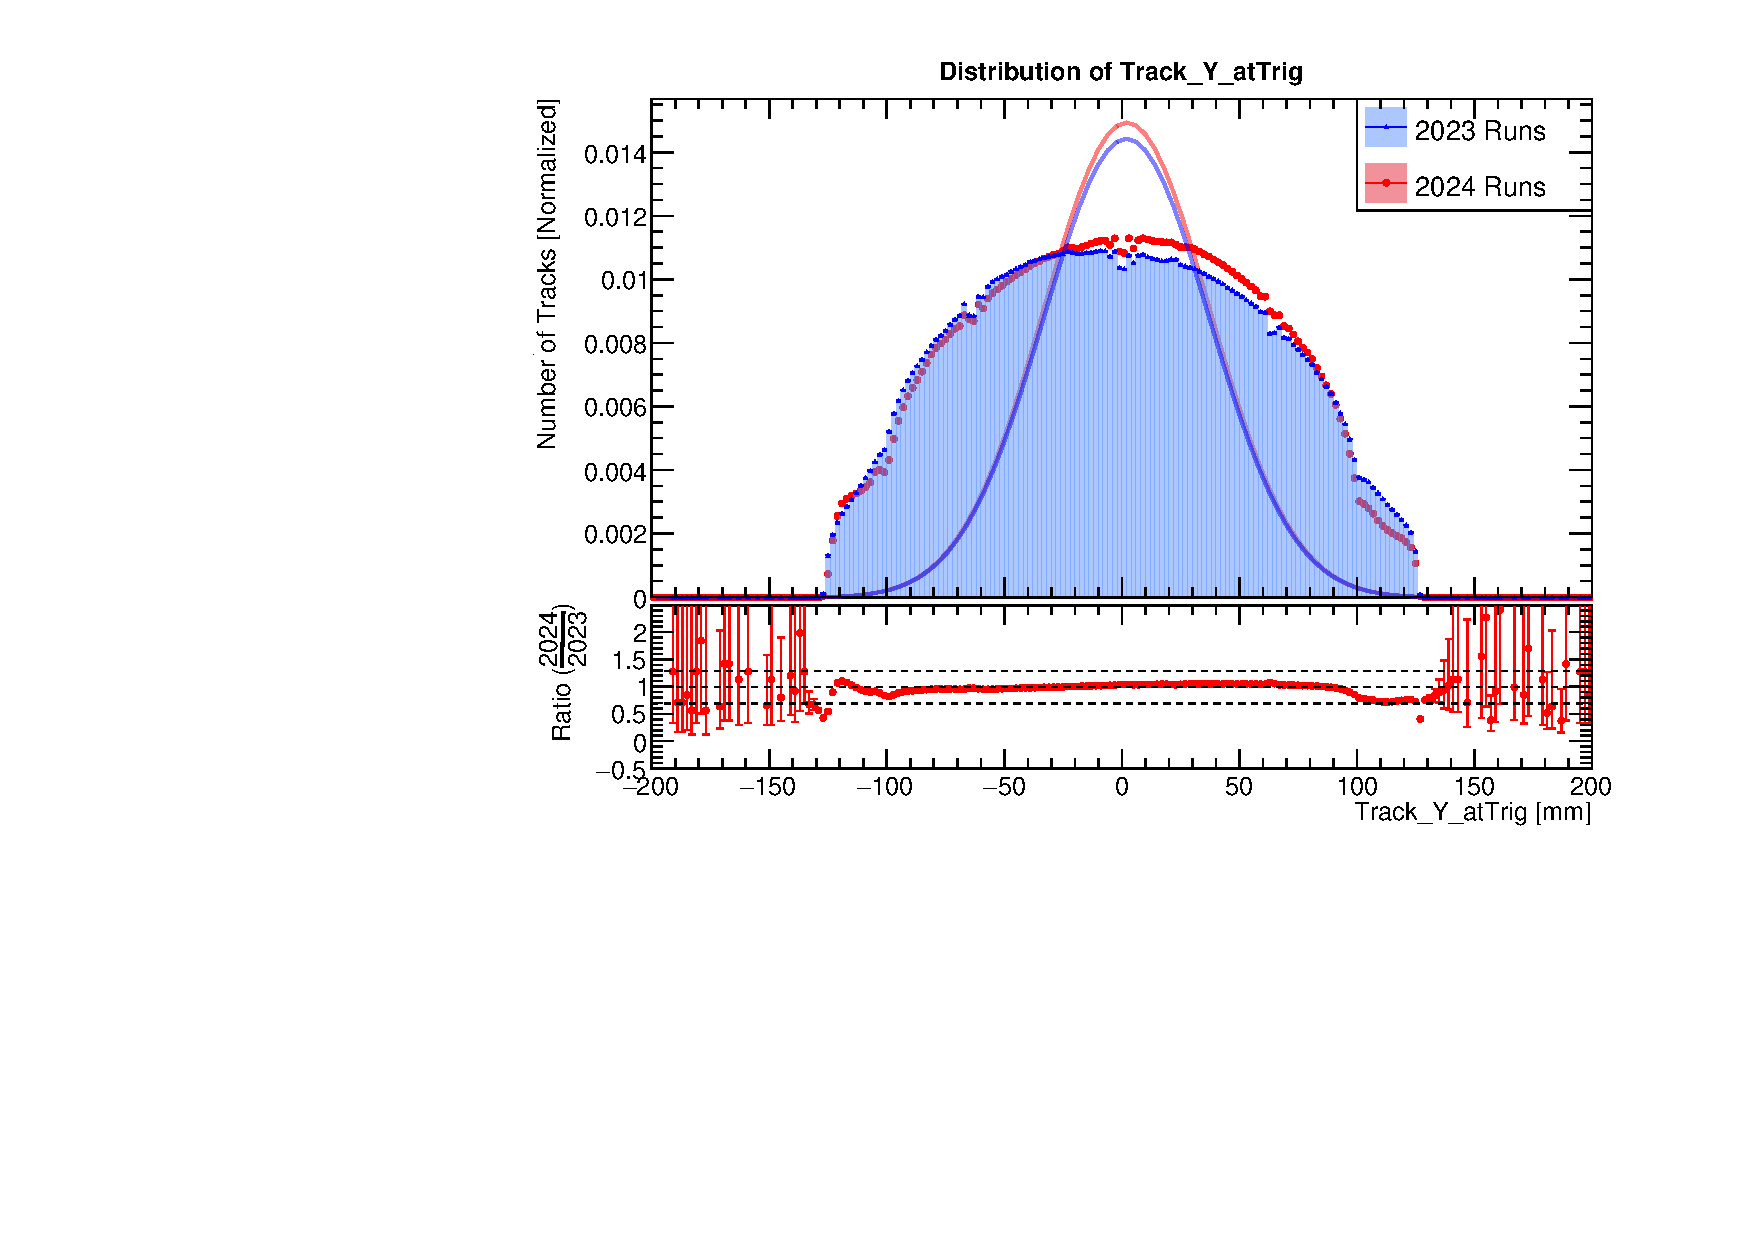
\includegraphics[width=\linewidth] {\plots/Track_Y_atTrig.pdf}
                \caption{Track Position y at Trigger/Timing Station}
            \end{figure}
        \end{column}
    \end{columns}
\end{subframe}

\begin{frame}{Track Positions at Tracking Station 1}
    \begin{columns}
        \begin{column}{0.5\textwidth}
            \begin{figure}
                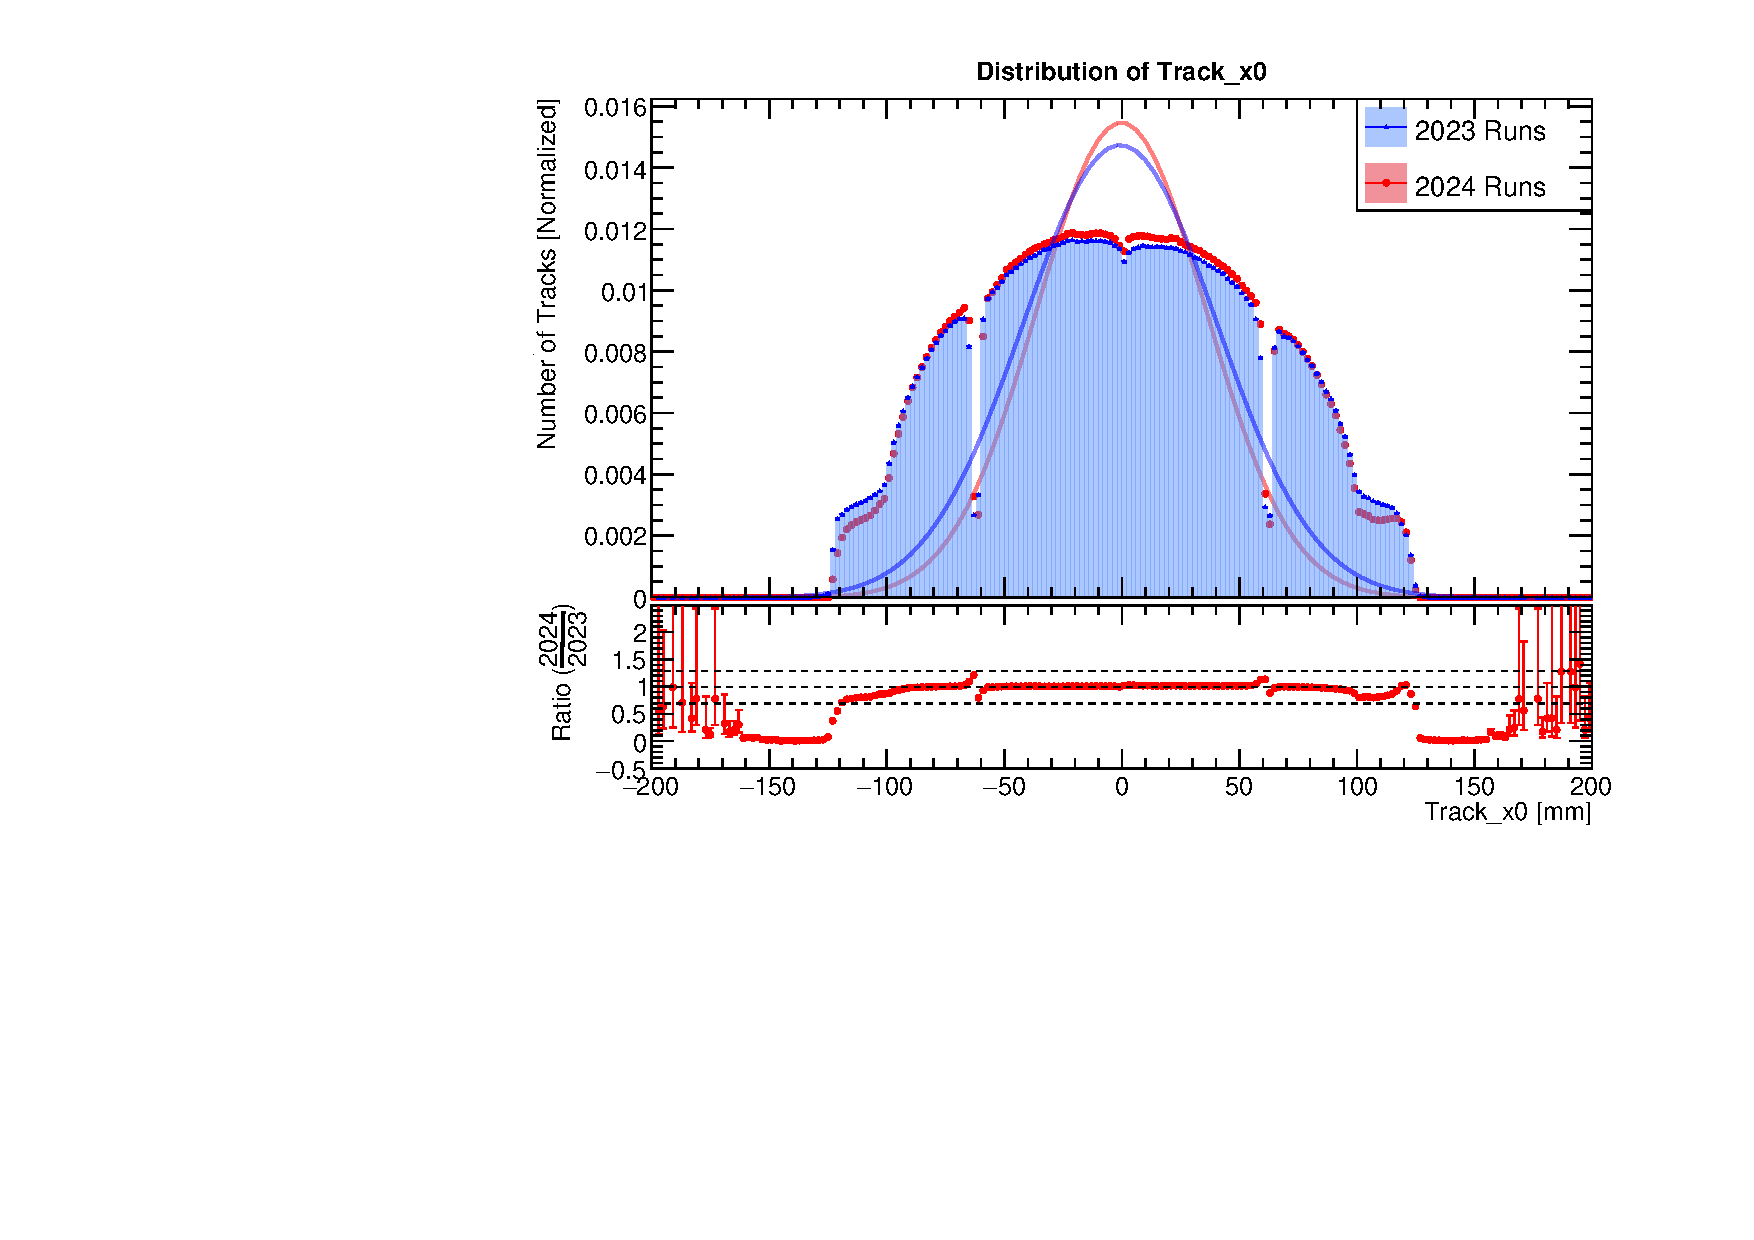
\includegraphics[width=\linewidth] {\plots/Track_x0.pdf}
                \caption{Track Position x at Tracking Station 1}
            \end{figure}
        \end{column}
        \begin{column}{0.5\textwidth}
            \begin{figure}
                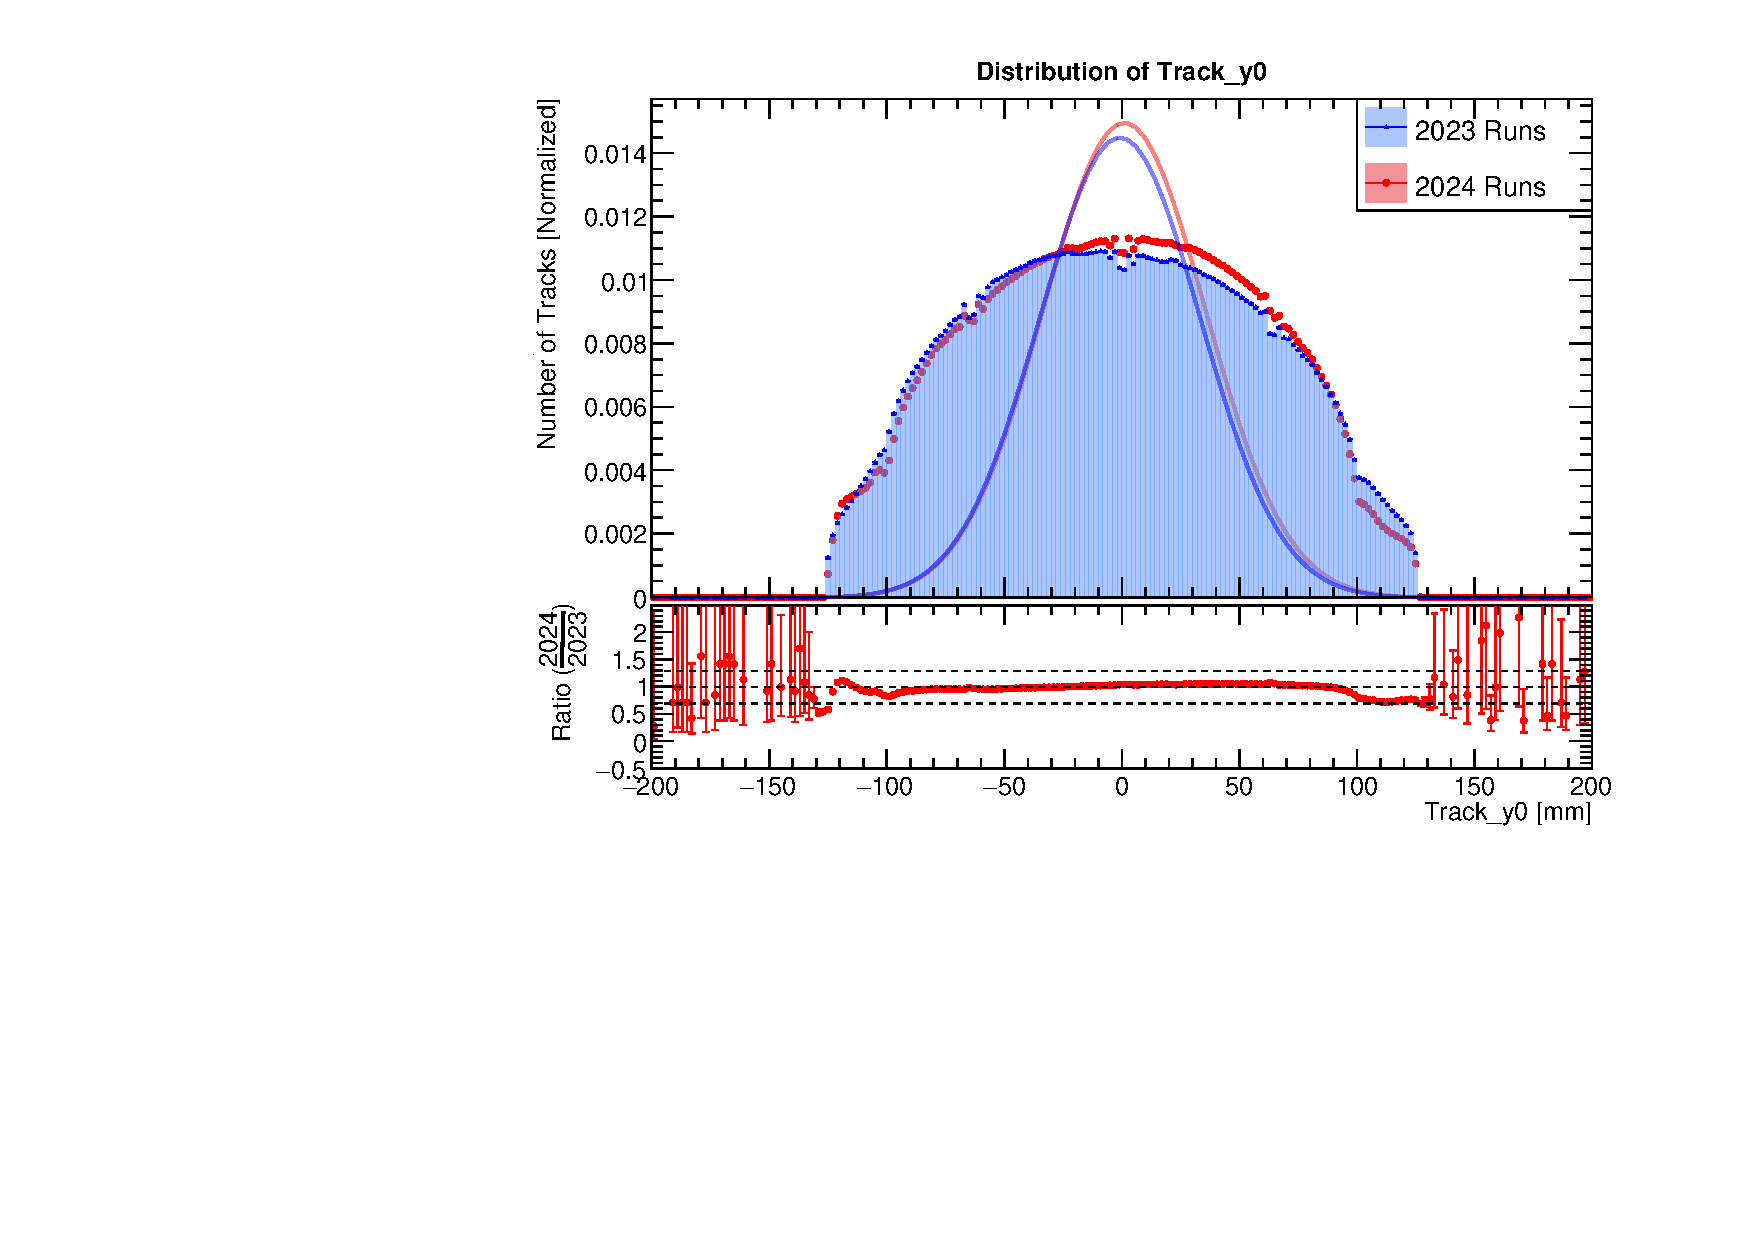
\includegraphics[width=\linewidth] {\plots/Track_y0.pdf}
                \caption{Track Position y at Tracking Station 1}
            \end{figure}
        \end{column}
    \end{columns}
    Only qualitative difference from the VetoNu plots are the sharper peaks here which are from the cut off at 125 mm.
    And the dips in the x-distributions at around 60mm are from the geometry of the tracking stations.
\end{frame}

\begin{frame}{Track Positions at Tracking Station 2}
    \begin{columns}
        \begin{column}{0.5\textwidth}
            \begin{figure}
                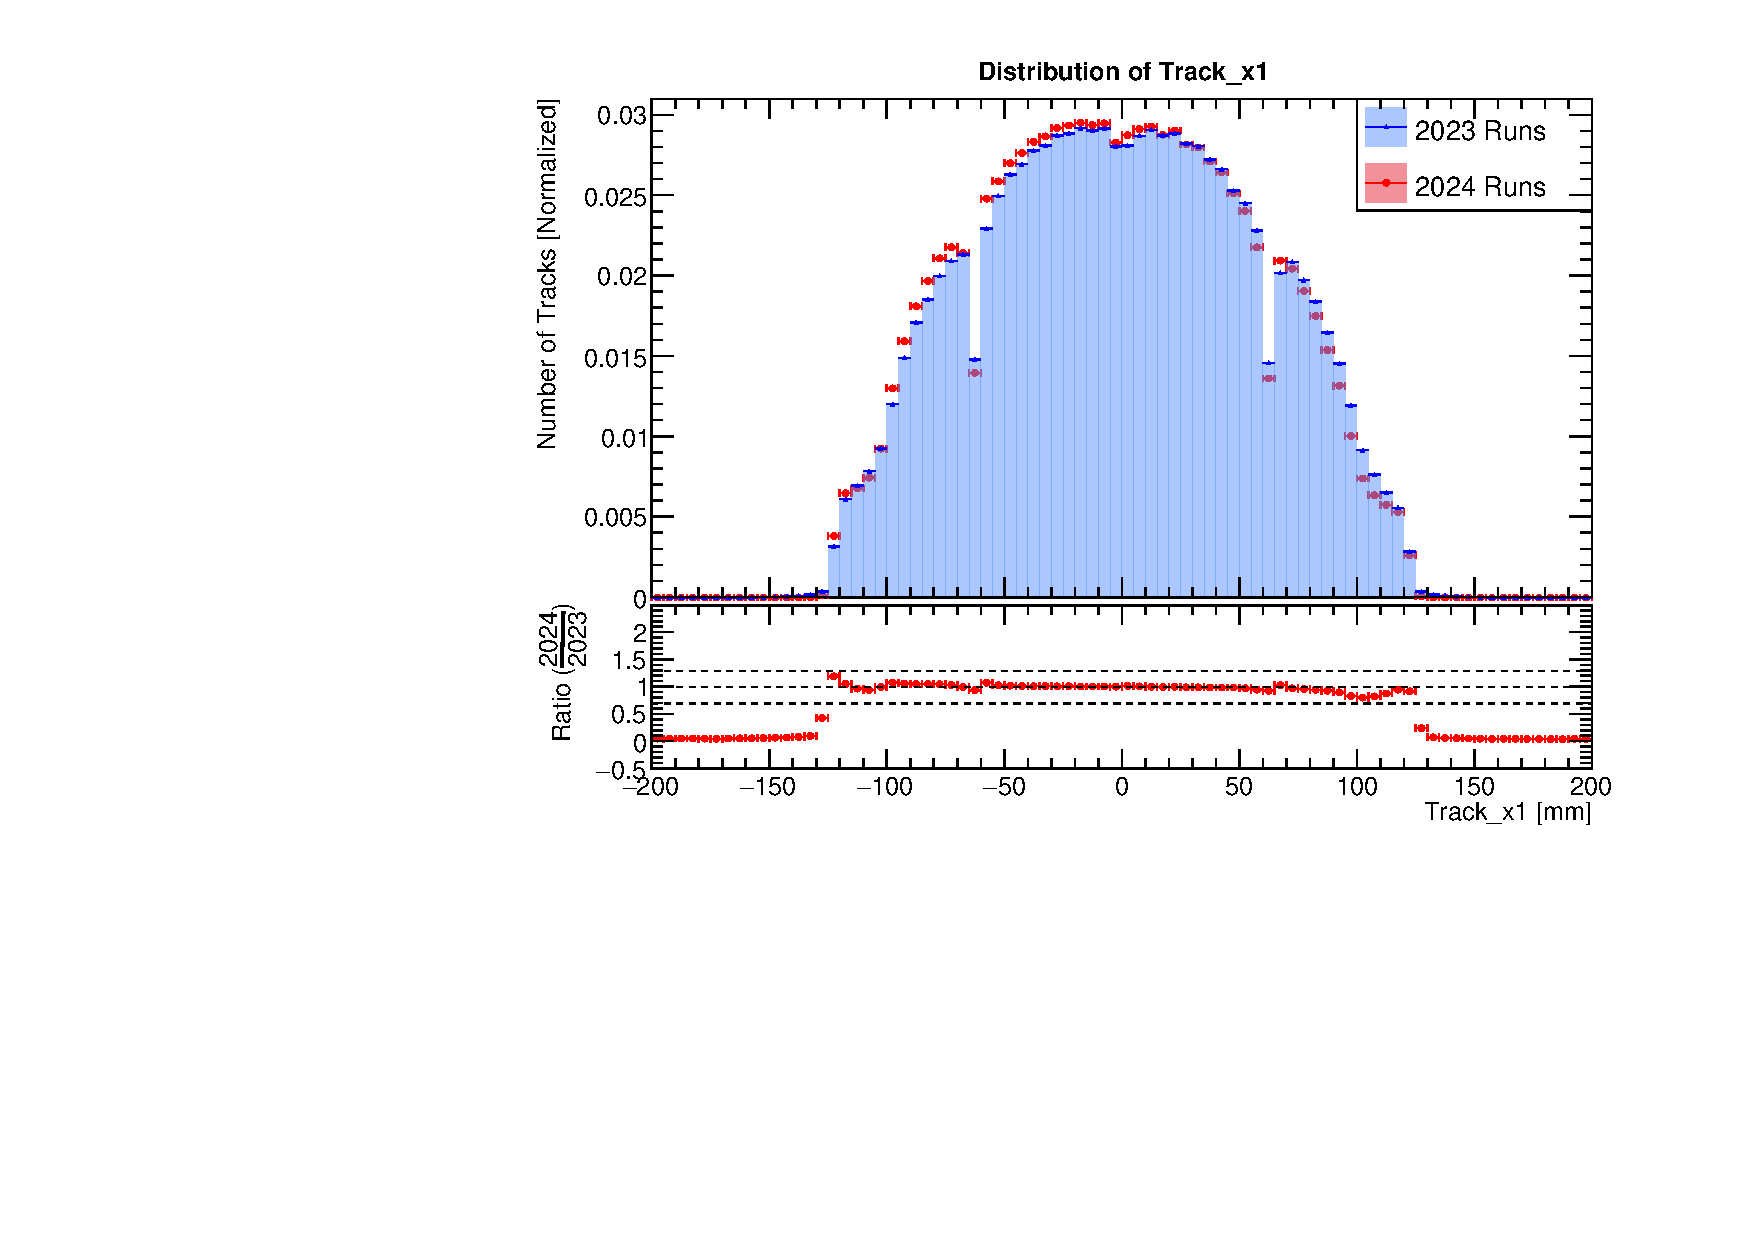
\includegraphics[width=\linewidth] {\plots/Track_x1.pdf}
                \caption{Track Position x at Tracking Station 2}
            \end{figure}
        \end{column}
        \begin{column}{0.5\textwidth}
            \begin{figure}
                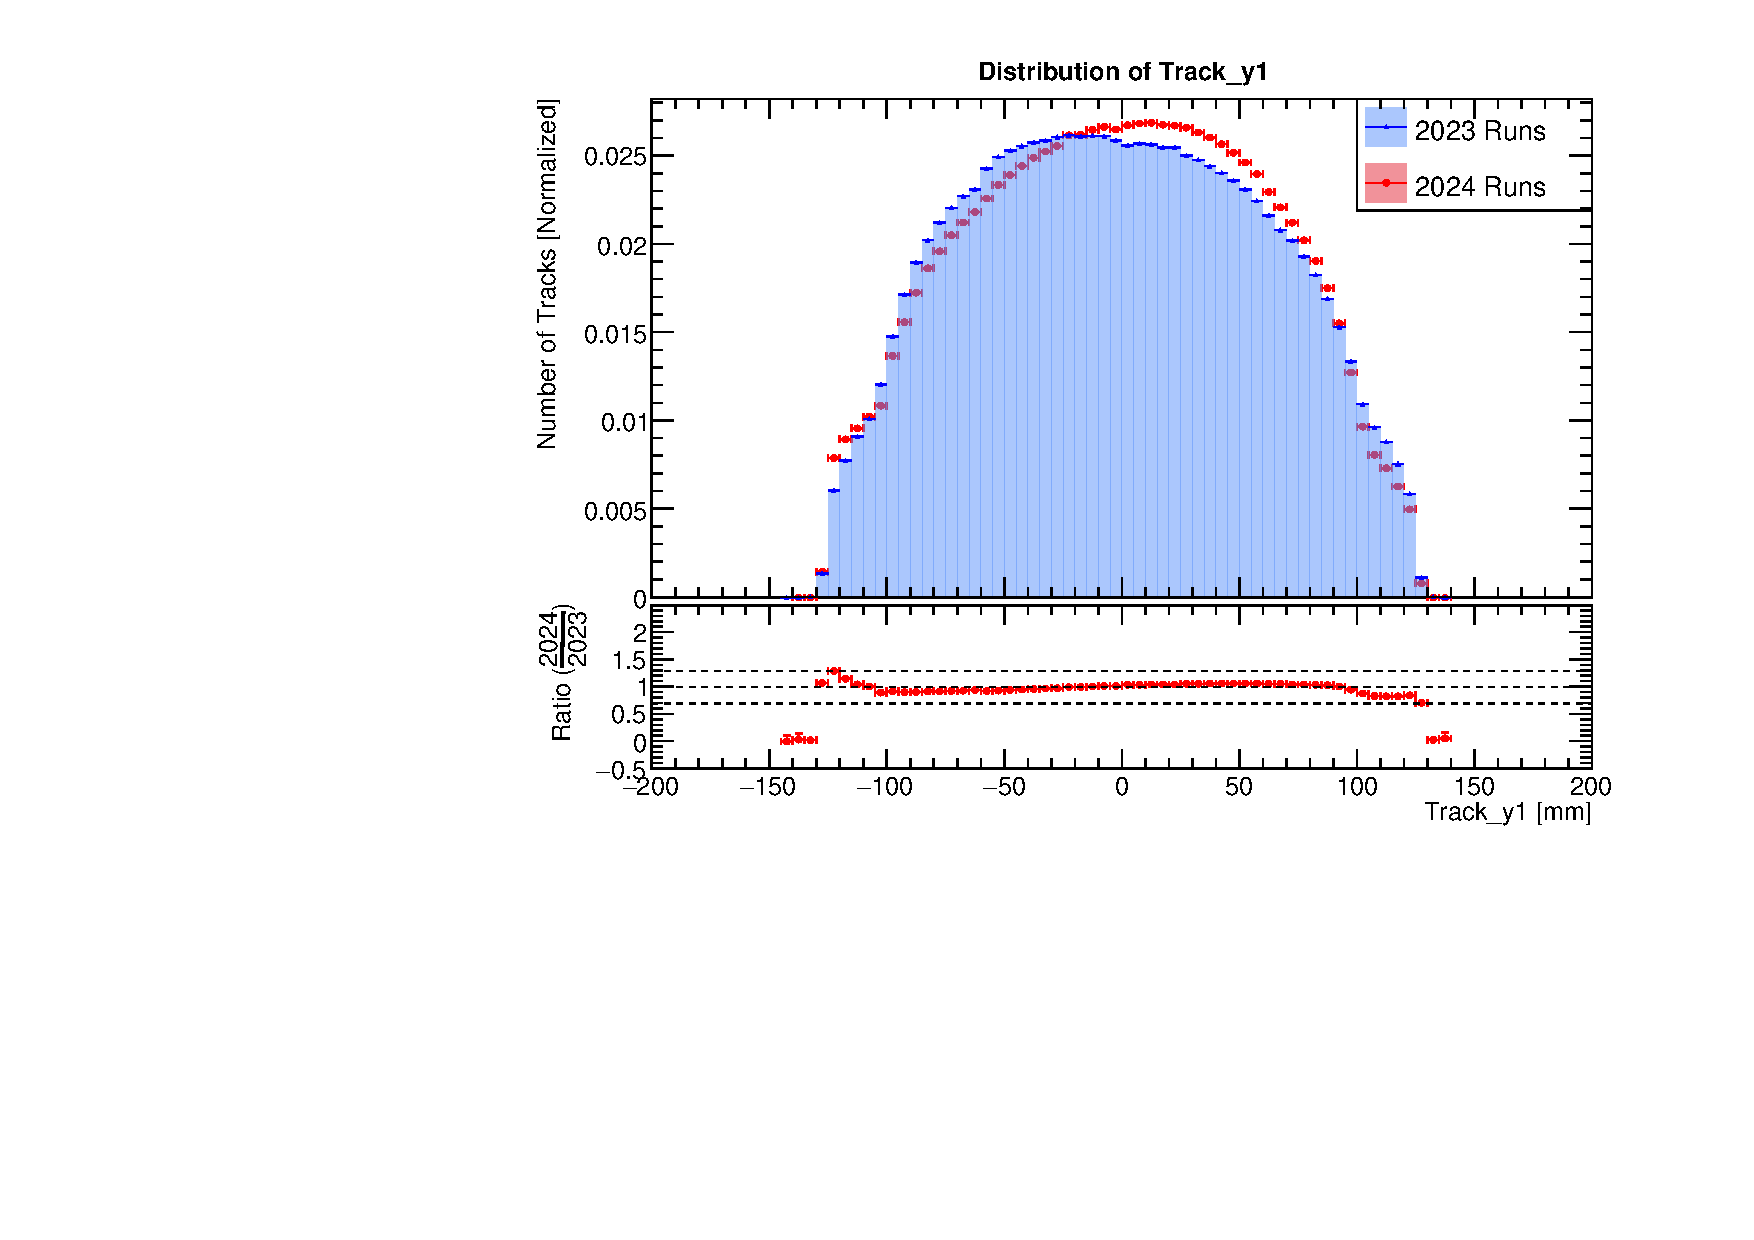
\includegraphics[width=\linewidth] {\plots/Track_y1.pdf}
                \caption{Track Position y at Tracking Station 2}
            \end{figure}
        \end{column}
    \end{columns}
\end{frame}

\begin{subframe}{Track Positions at Preshower 1 [SKIP]}
    \begin{columns}
        \begin{column}{0.5\textwidth}
            \begin{figure}
                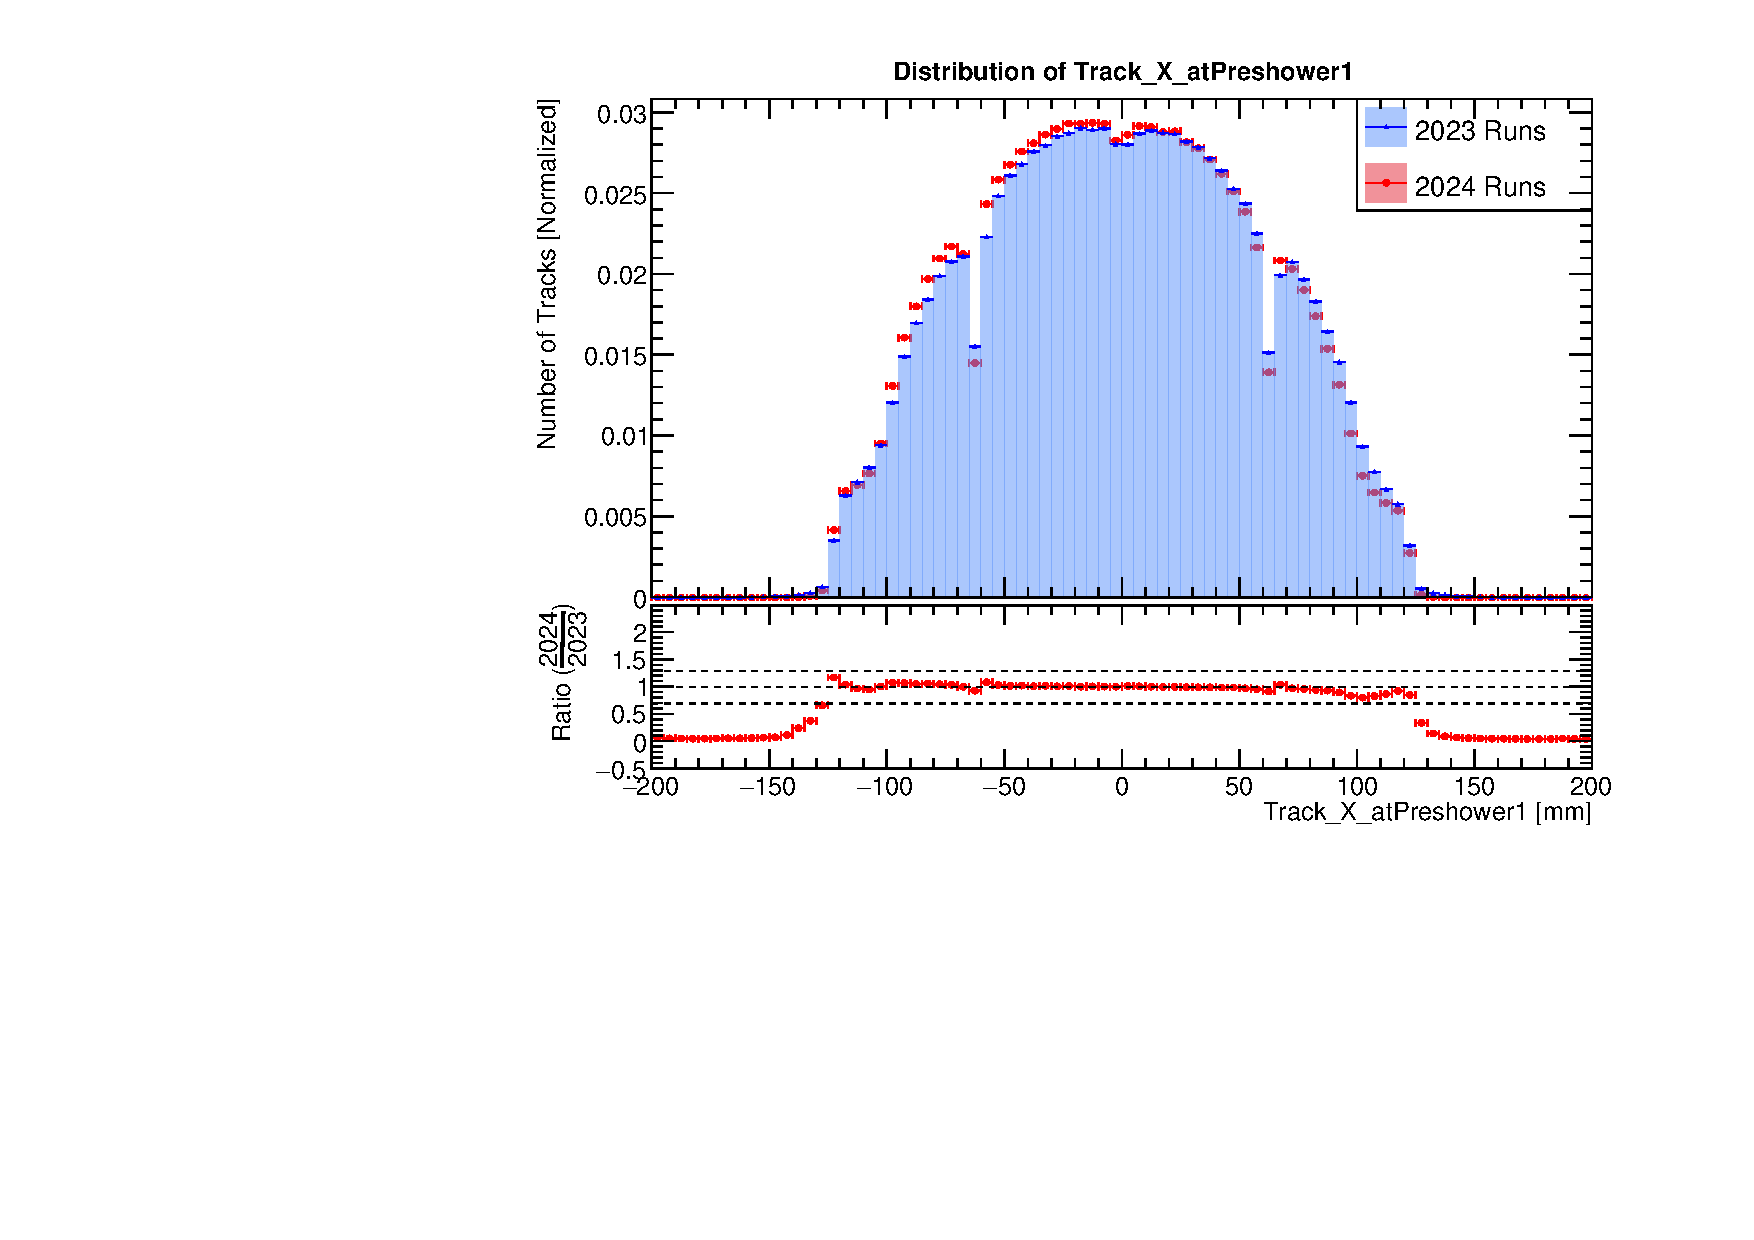
\includegraphics[width=\linewidth] {\plots/Track_X_atPreshower1.pdf}
                \caption{Track Position x at Preshower 1}
            \end{figure}
        \end{column}
        \begin{column}{0.5\textwidth}
            \begin{figure}
                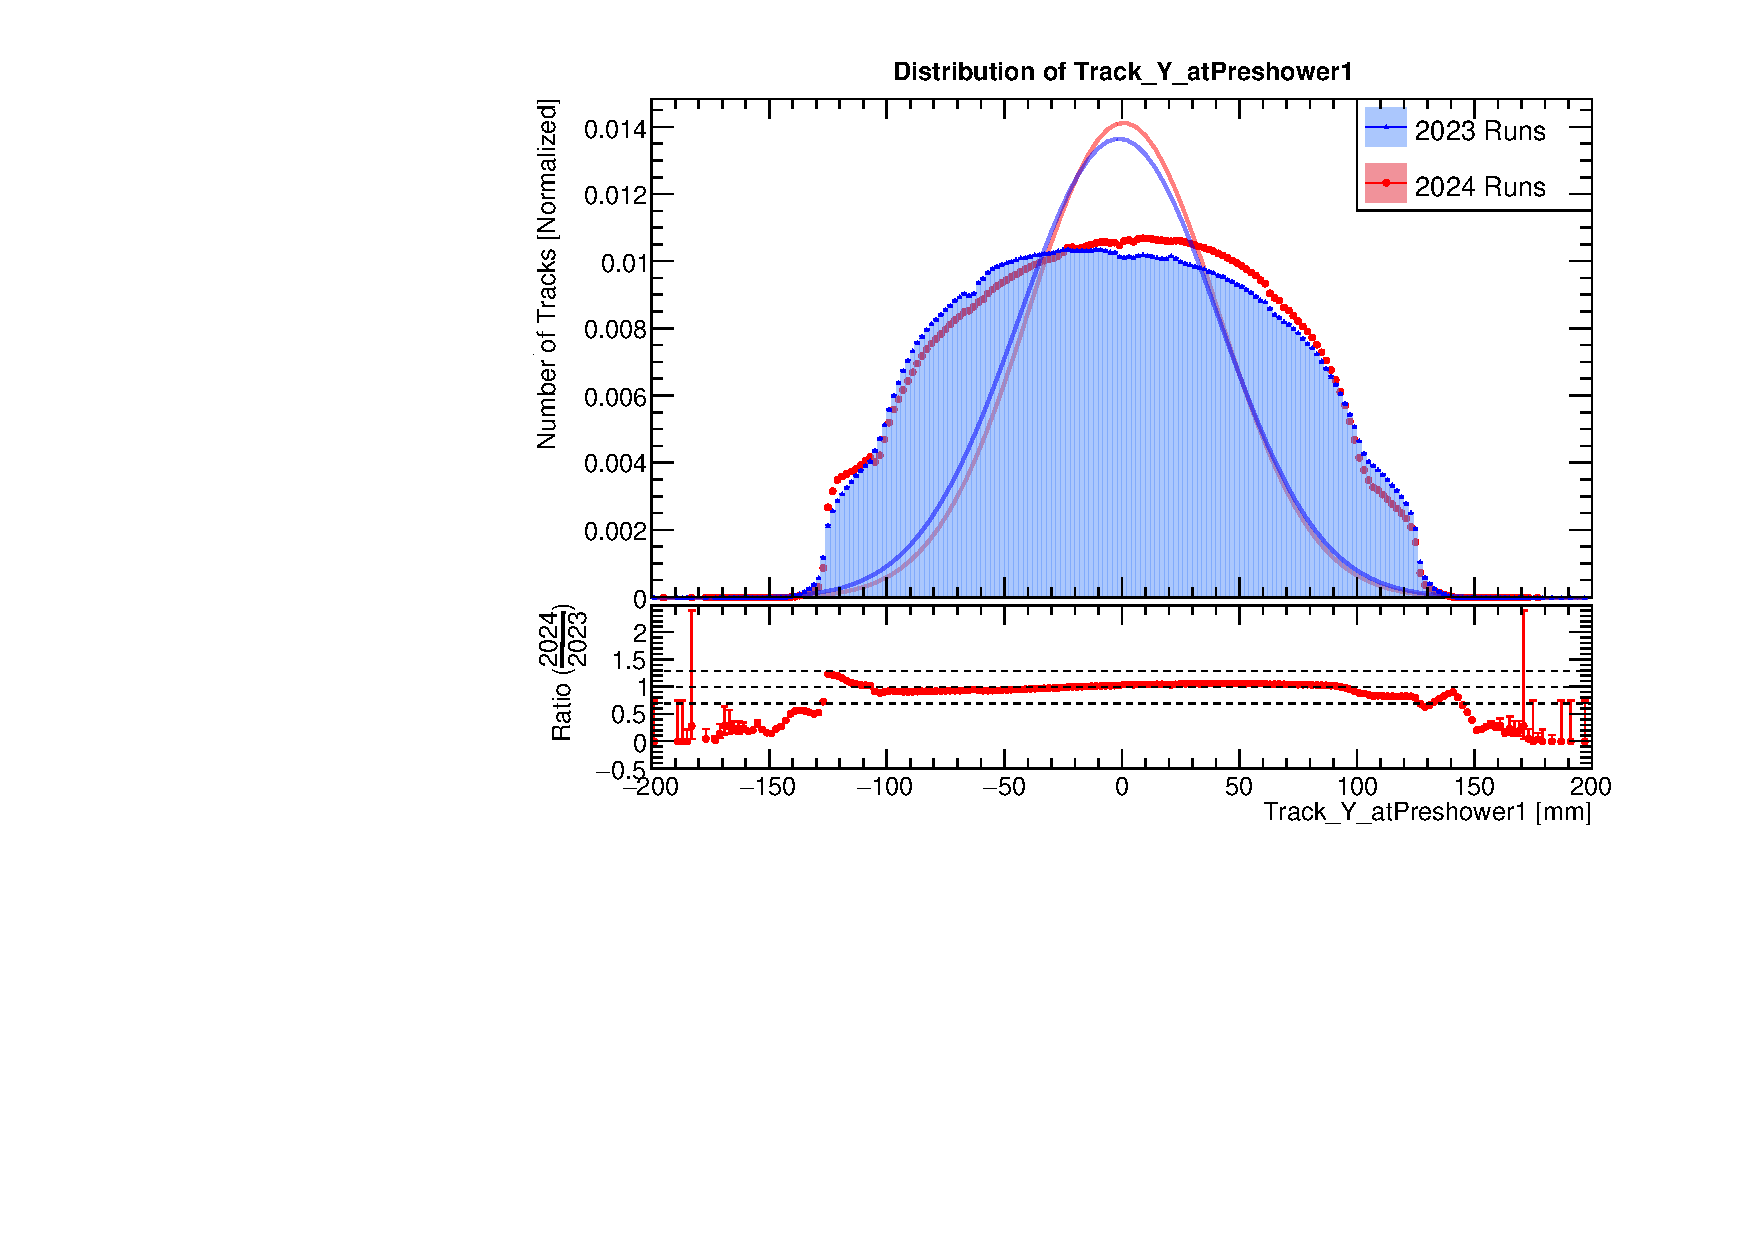
\includegraphics[width=\linewidth] {\plots/Track_Y_atPreshower1.pdf}
                \caption{Track Position y at Preshower 1}
            \end{figure}
        \end{column}
    \end{columns}
\end{subframe}

\begin{subframe}{Track Positions at Preshower 2 [SKIP]}
    \begin{columns}
        \begin{column}{0.5\textwidth}
            \begin{figure}
                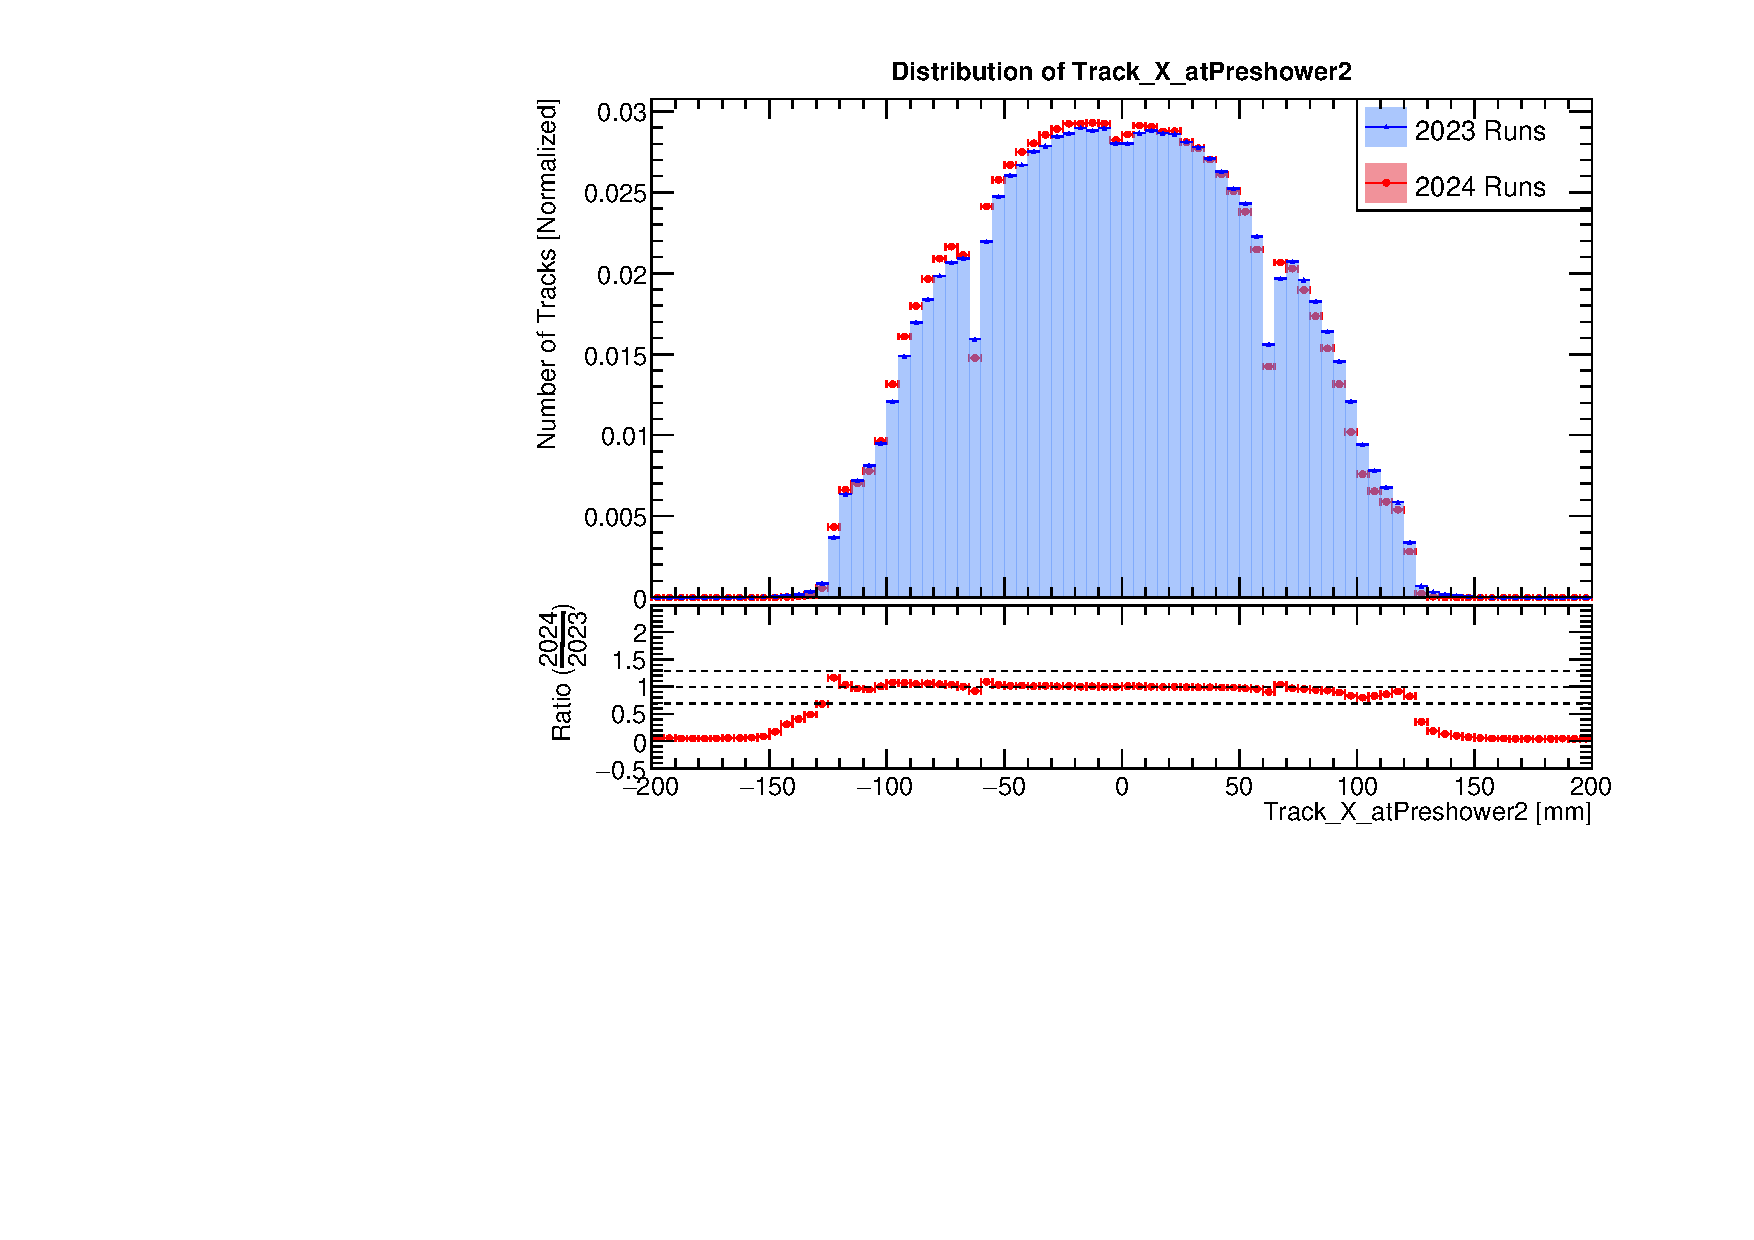
\includegraphics[width=\linewidth] {\plots/Track_X_atPreshower2.pdf}
                \caption{Track Position x at Preshower 2}
            \end{figure}
        \end{column}
        \begin{column}{0.5\textwidth}
            \begin{figure}
                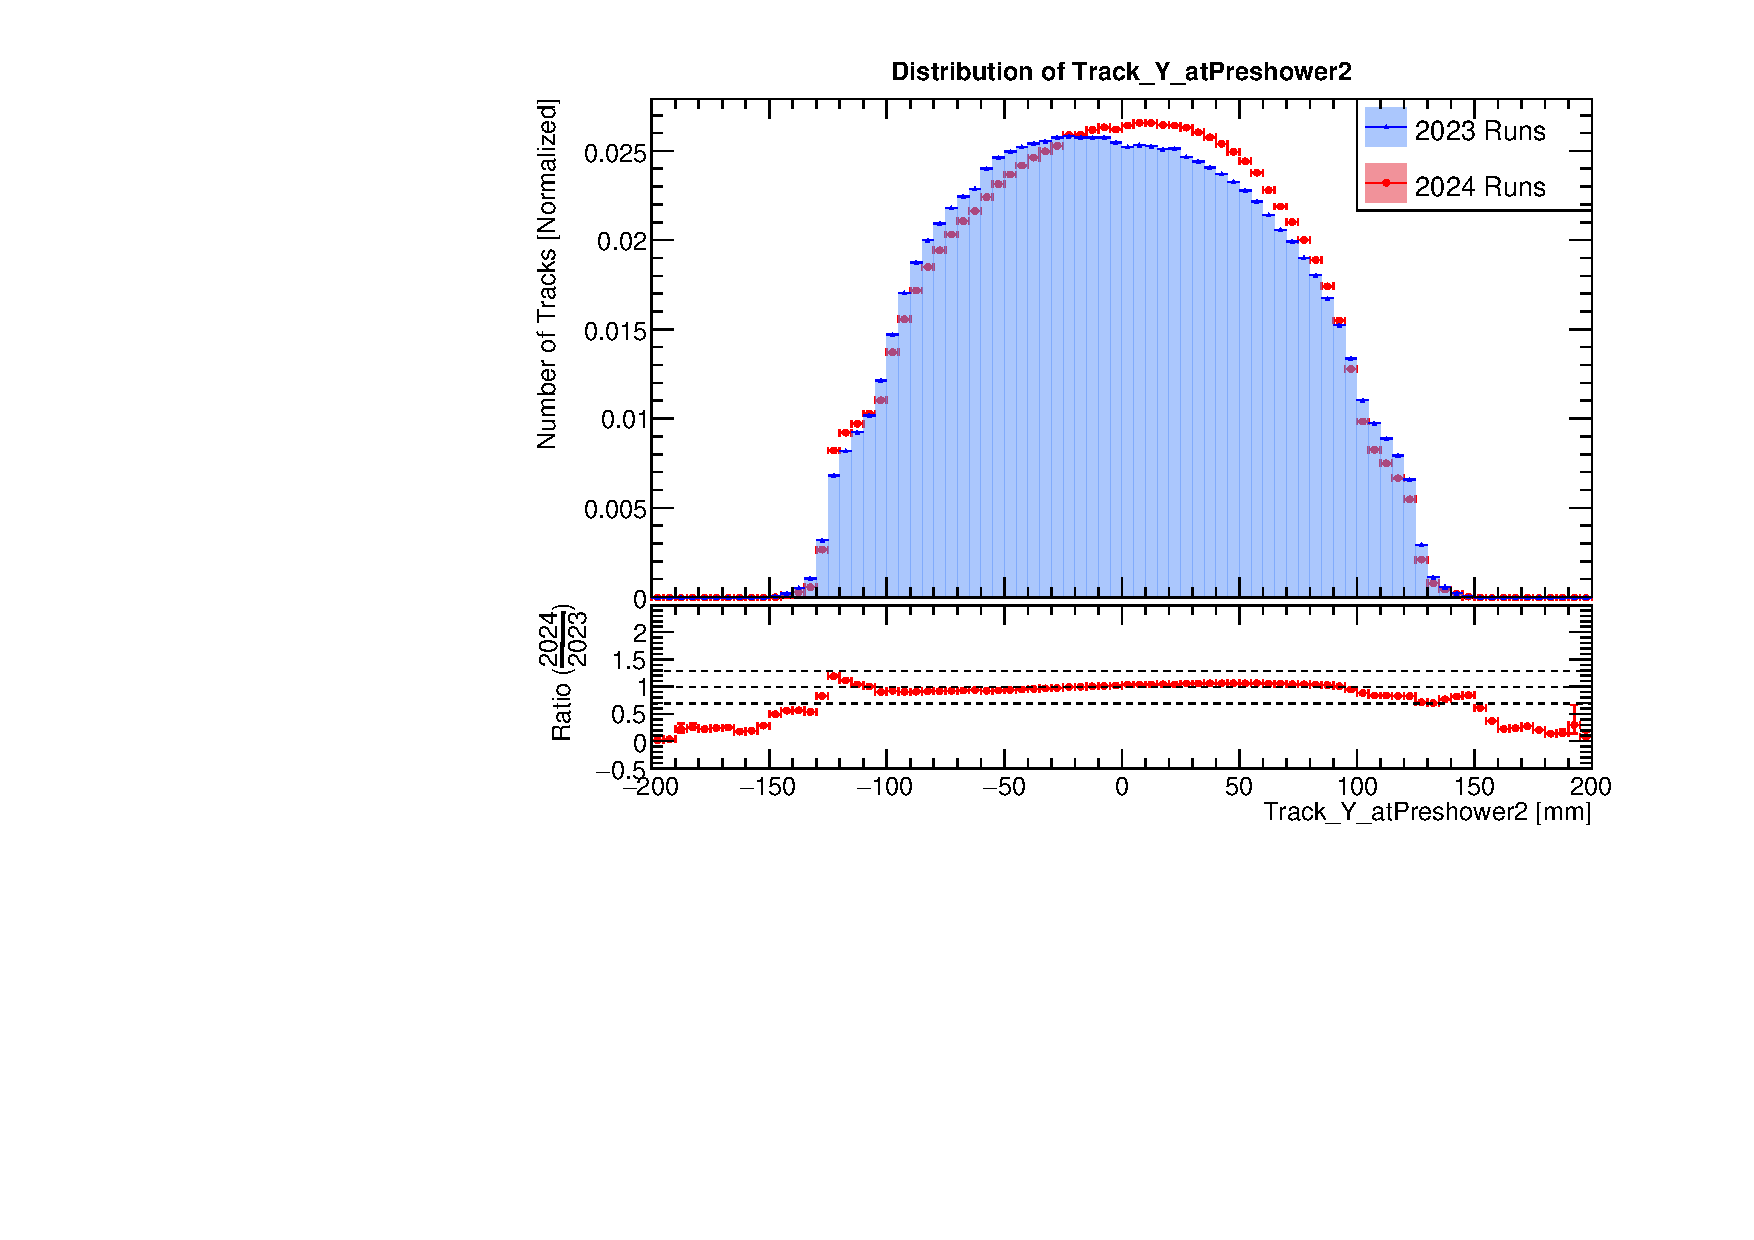
\includegraphics[width=\linewidth] {\plots/Track_Y_atPreshower2.pdf}
                \caption{Track Position y at Preshower 2}
            \end{figure}
        \end{column}
    \end{columns}
\end{subframe}

\begin{frame}{Track Positions at Calo}
    \begin{columns}
        \begin{column}{0.5\textwidth}
            \begin{figure}
                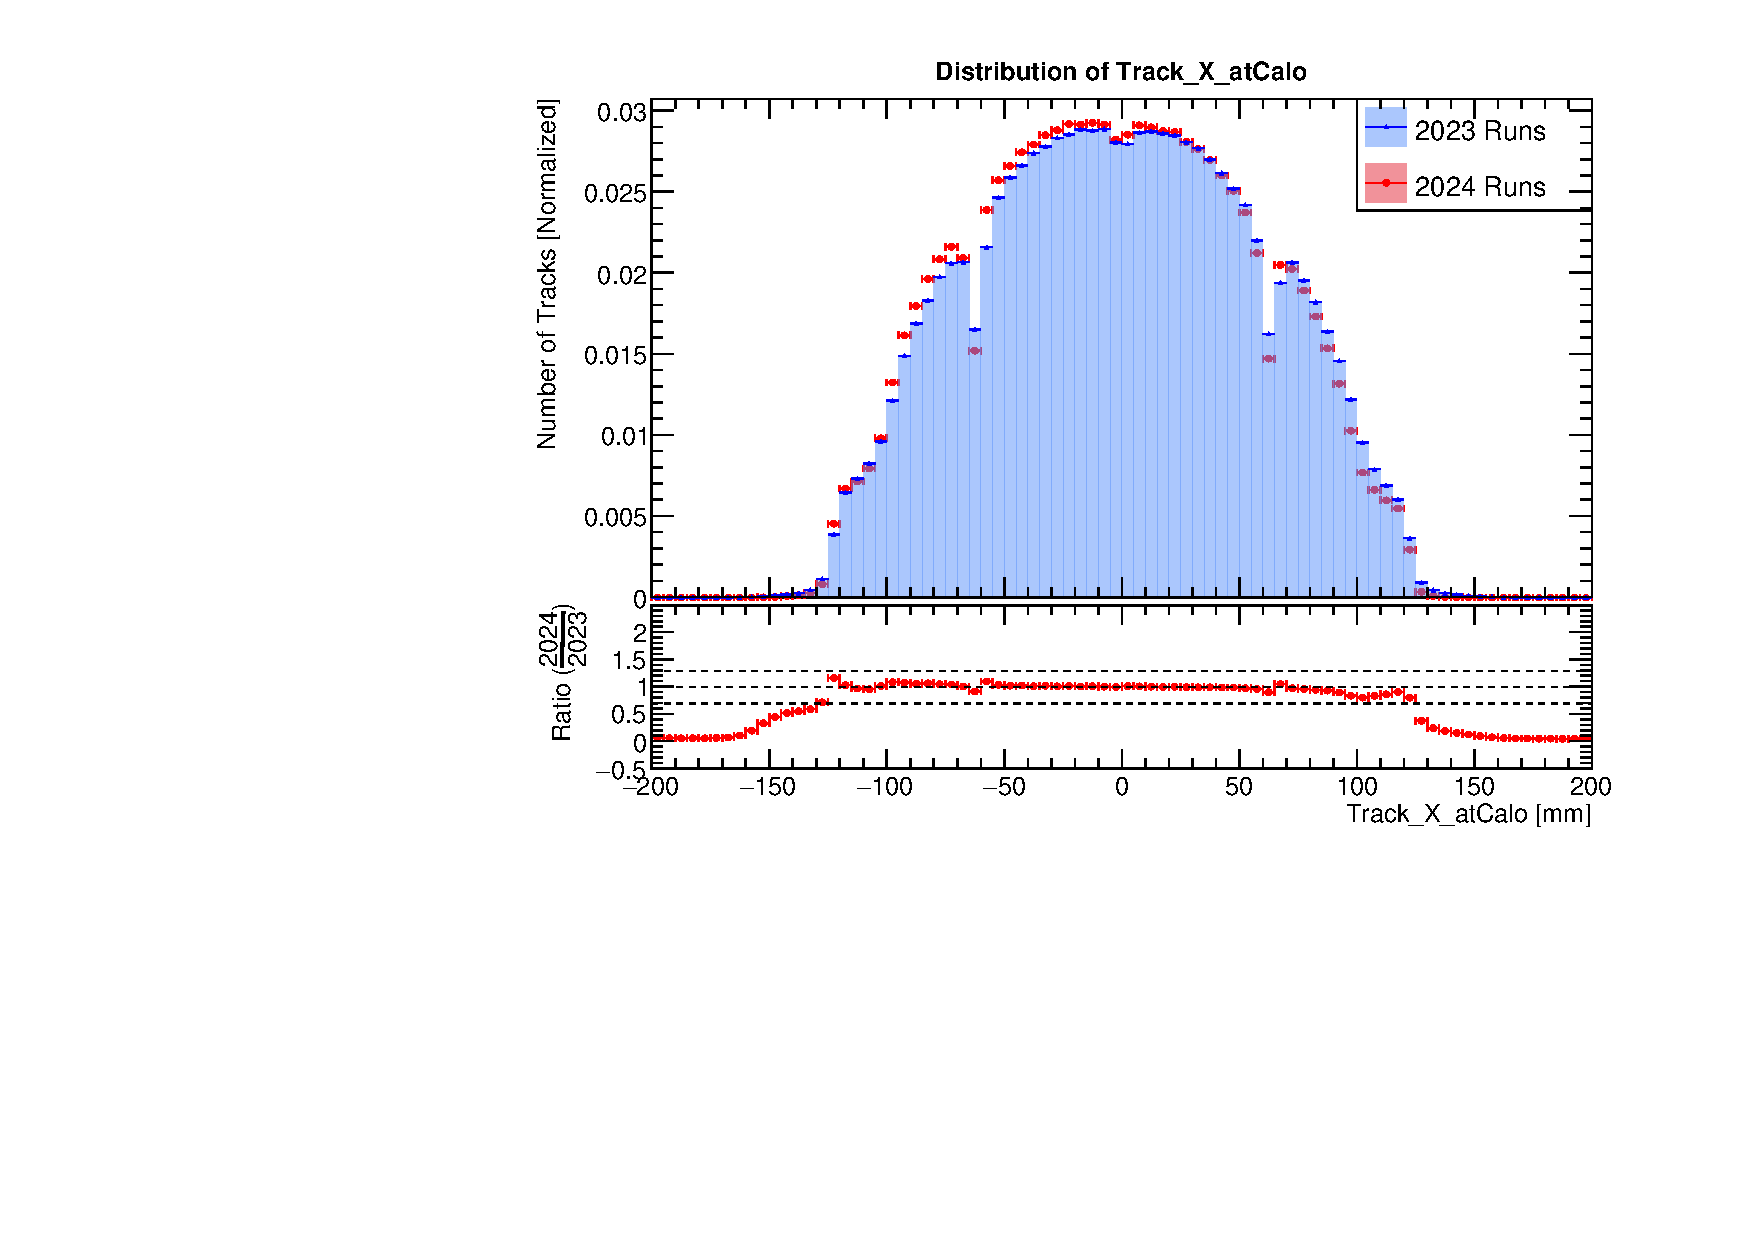
\includegraphics[width=\linewidth] {\plots/Track_X_atCalo.pdf}
                \caption{Track Position x at Calo}
            \end{figure}
        \end{column}
        \begin{column}{0.5\textwidth}
            \begin{figure}
                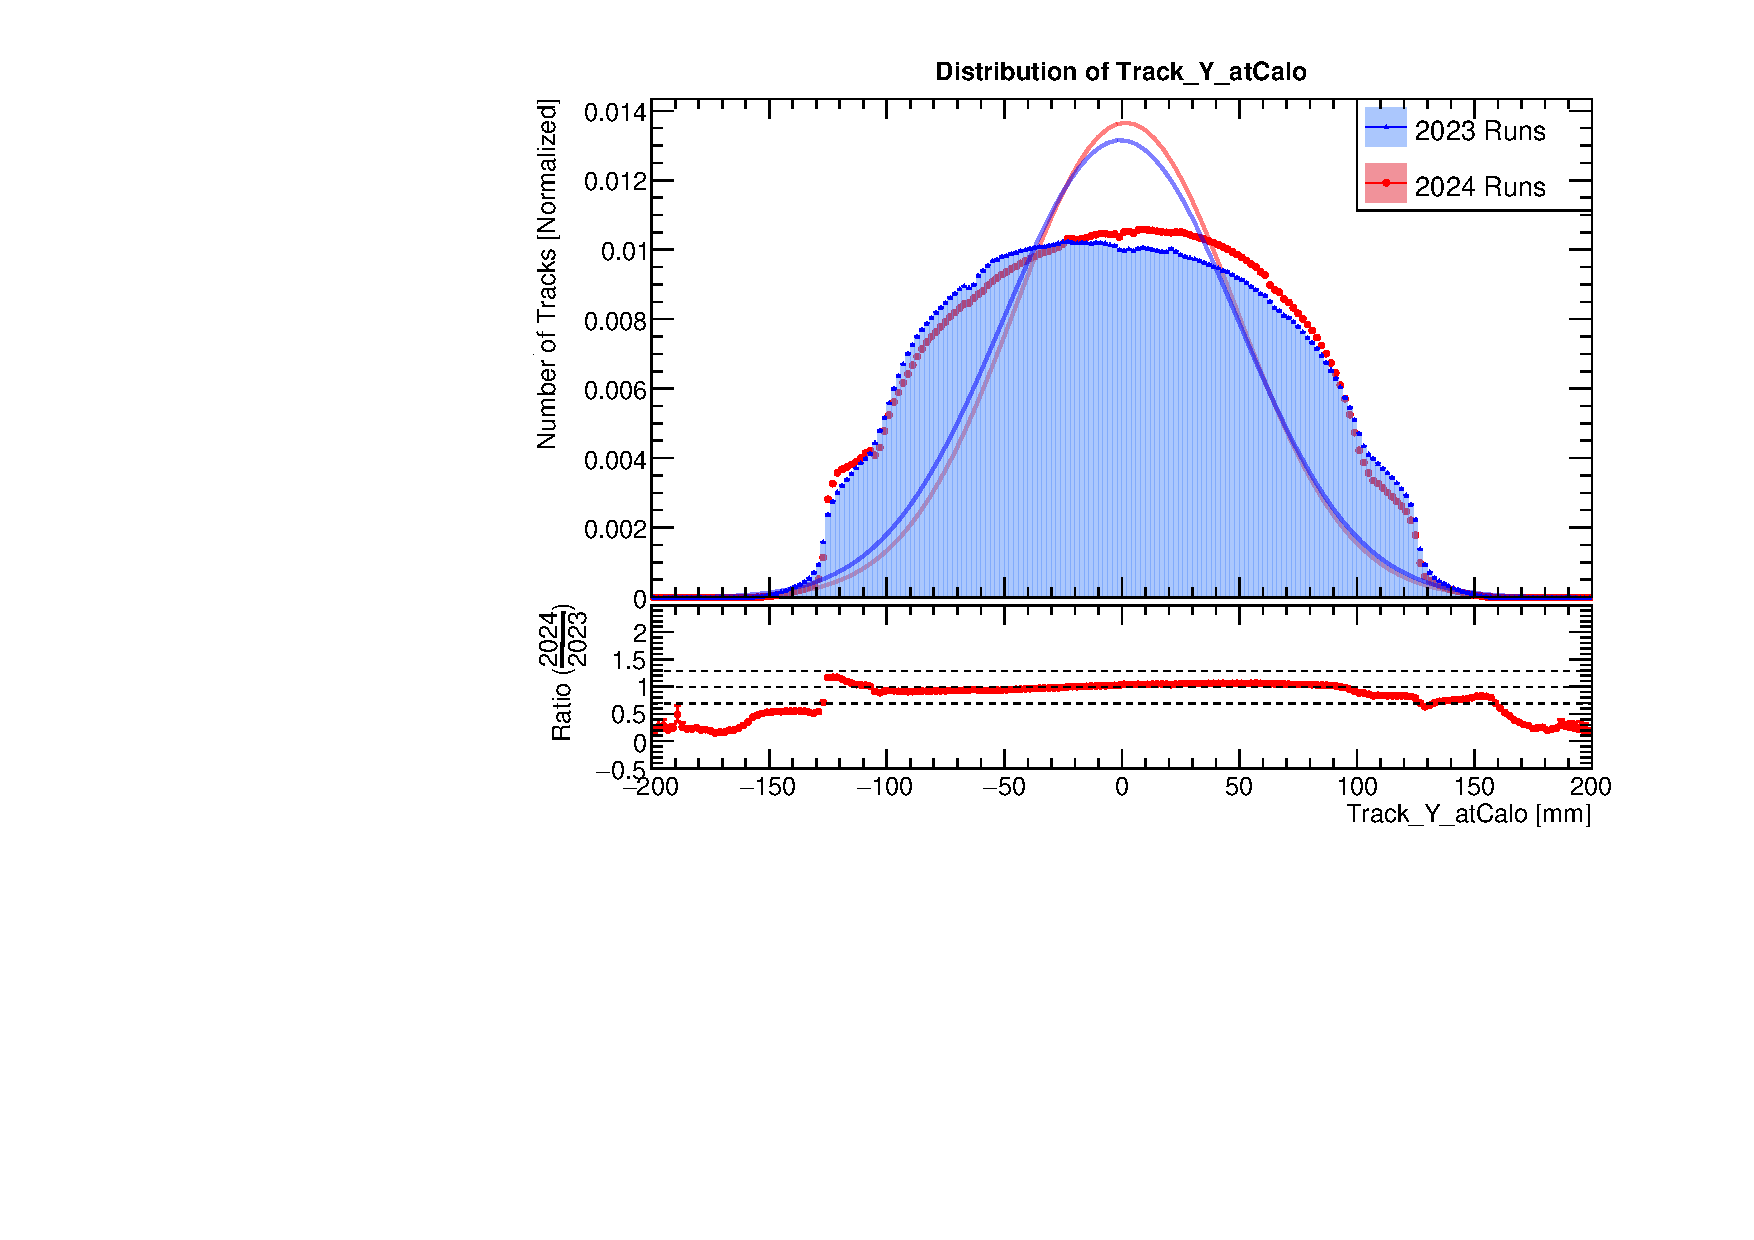
\includegraphics[width=\linewidth] {\plots/Track_Y_atCalo.pdf}
                \caption{Track Position y at Calo}
            \end{figure}
        \end{column}
    \end{columns}
\end{frame}

\begin{frame}{Track Positions at Max Radius}
    \begin{columns}
        \begin{column}{0.5\textwidth}
            \begin{figure}
                \includegraphics[width=\linewidth] {\plots/Track_X_atMaxRadius.pdf}
                \caption{}
            \end{figure}
        \end{column}
        \begin{column}{0.5\textwidth}
            \begin{figure}
                \includegraphics[width=\linewidth] {\plots/Track_Y_atMaxRadius.pdf}
                \caption{}
            \end{figure}
        \end{column}
    \end{columns}
\end{frame}